 \documentclass[book.tex]{subfiles}
\begin{document}
\chapter{Hardware}
\label{chapter_hardware}
To study the IBM PC, it is easiest to first break it down to small parts. Six sub-systems form a pipeline: Inputs, CPU, RAM, Disk, Video, and Audio.\\
\begin{figure}[H]
\centering
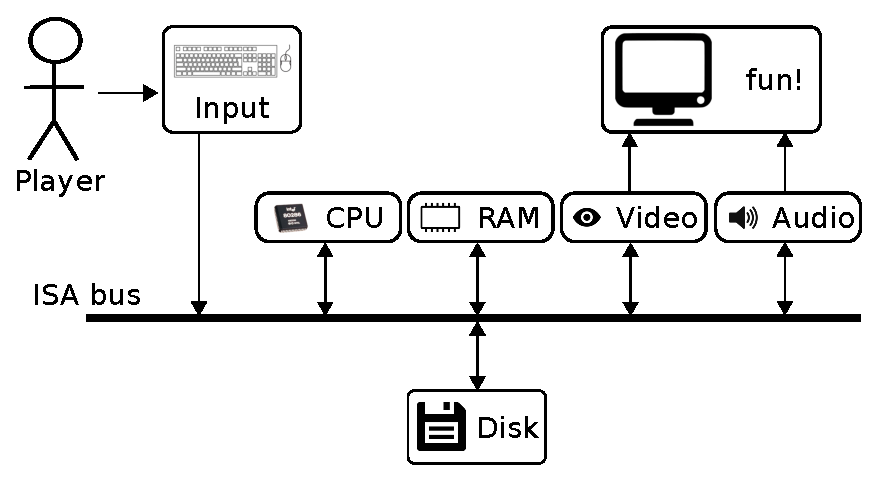
\includegraphics[width=\textwidth]{imgs/drawings/fun_pipeline.eps}
\caption{Hardware pipeline.}
\label{fig:digraph}
\end{figure}

A lot of friction was present since manufacturers had not embraced the gaming industry yet. Parts quality varied from  bad, terrible, to downright impossible to deal with.\\
\par

\begin{figure}[H]
\centering
\begin{tabularx}{\textwidth}{ X X  }
  \toprule
  \textbf{Stage} & \textbf{Quality} \\ \bottomrule
  RAM & Bearable \\ 
  Video & Impossible \\ 
  Audio & Very Poor \\ 
  Inputs & Ok \\ 
  CPU & Very Poor \\ 
  Disk & Ok \\ \bottomrule
\end{tabularx}
\caption{Component quality for a game engine.}
\end{figure}



\section{CPU: Central Processing Unit}
  


  In 1989 around 15\% of the households owned a computer\footnote{https://www.statista.com/statistics/184685/percentage-of-households-with-computer-in-the-united-states-since-1984/}. The performance of these machines was so overwhelmingly determined by the CPU that a PC was referred to not by its brand or GPU\footnote{There was no GPU yet. The term was coined by Nvidia in 1999, who marketed the GeForce 256 as "the world's first GPU", or Graphics Processing Unit.}, but by the main chip inside. If a PC had an Intel 8088 or equivalent, it was called a "XT" . If it had an Intel 80286, it was a "286" or "AT".\\
\subsection{Overview}
  Intel released the 8086 in 1979, which was the first microchip of the successful x86 family line. One year later, in 1979, it released the 8088 which was a variant of the 8086. The main difference between the two is that there are only eight data lines for the external data bus in the 8088 instead of the 8086's 16 lines.  However, because it retained the full 16-bit internal registers and the 20-bit address bus, the 8088 ran 16-bit software and was capable of addressing a full 1MB of RAM. IBM chose the 8088 over the 8086 for its original PC/XT, because Intel offered a better price for the former and could supply more units. \\
  \par
  In 1982 Intel released the 80286 microchip. A typical 8088 chip was running at 4.77Mhz, where the 80286 was running at 8Mhz and later versions at 12-16Mhz. The 80286 was employed for the IBM PC/AT, introduced in 1984, and then widely used in most PC/AT compatible computers until the early 1990s. Commander Keen could run on a 8088, but an Intel 286 was recommended.\\   

\par


\begin{figure}[H]
\centering
  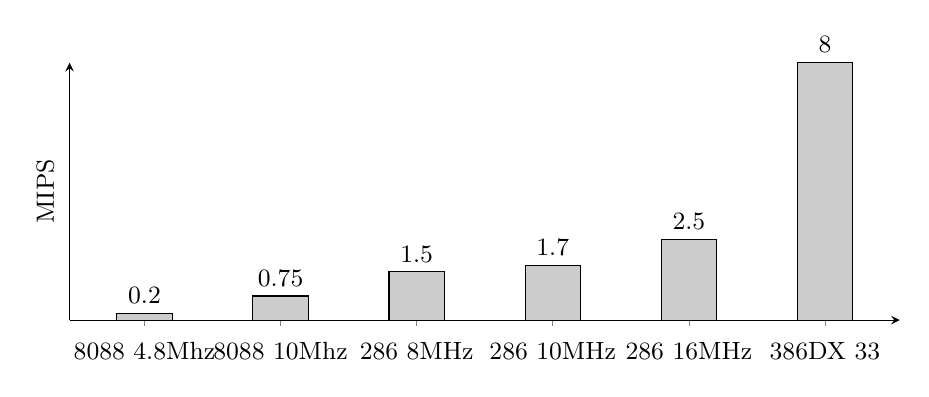
\begin{tikzpicture}[font=\small]
    \begin{axis}[
      width=1.0\textwidth,
      height=0.4\textwidth,
      ybar,
      bar width=20pt,
      ylabel={MIPS},
      ymin=0,
      ytick=\empty,
      xtick=data,
      axis x line=bottom,
      axis y line=left,
      enlarge x limits=0.11,
      symbolic x coords={8088 4.8Mhz, 8088 10Mhz, 286 8MHz,286 10MHz,286 16MHz,386DX 33},
      xticklabel style={anchor=base,yshift=-\baselineskip},
      nodes near coords={\pgfmathprintnumber\pgfplotspointmeta}
    ]
      \addplot[fill=black!20,draw=black] coordinates {
		(8088 4.8Mhz,0.2)      	
      	(8088 10Mhz,0.75)
        (286 8MHz,1.5)
        (286 10MHz,1.7)
        (286 16MHz,2.5)
        (386DX 33,8)
      };
    \end{axis}
   
   \end{tikzpicture}
   \caption{Comparison\protect\footnotemark of CPUs with MIPS}
 \end{figure}
 \par
 % \addtocounter{footnote}{0}
  \footnotetext{Roy Longbottom's PC Benchmark Collection: http://www.roylongbottom.org.uk/mips.htm.}
   % \stepcounter{footnote}
 \par
  \textbf{\underline{Trivia :}} A modern processor such as the Intel Core i7 3.33 GHz operates at close to 180,000 MIPS.\\
  \par

\subsection{The Intel 80286}
  \begin{wrapfigure}[7]{r}{0.3\textwidth}
\centering
\vspace{-10pt}

\includegraphics[width=.3\textwidth]{imgs/drawings/intel_logo.eps}
\end{wrapfigure}
\par
The Intel 80286 chip, first introduced in 1982, is the CPU behind the original IBM PC AT (Advanced Technology). Other computer makers manufactured what came to be known as IBM clones, with many of these manufacturers calling their systems AT-compatible or AT-class computers. \\
\par
When IBM developed the AT, it selected the 286 as the basis for the new system because the chip provided compatibility with the 8088 used in the PC and the XT. Therefore, software written for those chips should run on the 286. The 286 chip is many times faster than the 8088 used in the XT, and at the time it offered a major performance boost to PCs used in businesses. The processing speed, or throughput, of the original AT (which ran at 6MHz) is five times greater than that of the PC running at 4.77MHz.
286 systems are faster than their predecessors for several reasons. The main reason is that 286 processors are much more efficient in executing instructions. An average instruction takes 12 clock cycles on the 8086 or 8088, but takes an average of only 4.5 cycles on the 286 processor. Additionally, the 286 chip can handle up to 16 bits of data at a time through an external data bus twice the size of the 8088.\\
\par
The 286 chip has two modes of operation: real mode and protected mode. The two modes are distinct enough to make the 286 resemble two chips in one. In real mode, a 286 acts essentially the same as an 8086 chip and is fully compatible with the 8086 and 8088. In the protected mode of operation, the 286 was truly something new. In this mode, a program designed to take advantage of the chip's capabilities has access to 1GB of memory (including virtual memory). The 286 chip, however, can address only 16MB of hardware memory. A significant failing of the 286 chip is that it cannot switch from protected mode to real mode without a hardware reset (a warm reboot) of the system (It can, however, switch from real mode to protected mode without a reset).\\

\par
While the 8088 used a 3.0$\mu$m process, the 20286 used a 1.5$\mu$m process. The smaller process and increased surface (from 33mm$^2$ to 49mm$^2$) allowed Intel to pack 134,000 transistors on a 286 chip versus 29,000 on a 8088 chip.\\


\fullimage{286_layout_photo.png}
\par \vspace{-1pt}
% Below, a 1:1 scale of the 3.68cm x 3.68cm packaging next to a schematic showing the actual die inside.\\
\begin{minipage}{0.48\textwidth}
\centering
\scaledrawimage{3.68cm}{286_packaging.png} 

\end{minipage}
\hfill
\begin{minipage}{0.48\textwidth}
\centering
\scaledrawimage{3.68cm}{286_packaging_die.png}
\end{minipage}



 \pagebreak

\par Despite the apparent complexity, the 80286 can be summarized by functional units and a three-stage instruction pipeline.


\begin{figure}[H]
\centering
\includegraphics[width=\textwidth]{imgs/drawings/286_architecture.eps}
\caption{Internal block diagram of the 80286 processor}
\end{figure}
\par
The four functional units can be described by
\begin{itemize}
\item \textbf{address unit (AU)} is used to determine the physical addresses of instructions and operands which are stored in memory. The address lines derived by AU can be used to address different peripheral devices such as memory and I/O devices. 
\item \textbf{bus unit (BU)} interfaces the 80286 with memory and I/O devices. The bus unit is used to fetch instruction bytes from the memory and stores them in the prefetch queue.
\item \textbf{instruction unit (UI)} receives instructions from the prefetch queue and an instruction decoder decodes them one by one. The decoded instructions are latched onto a decoded instruction queue.
\item \textbf{execution unit (EU)} is responsible for executing the instructions received from the decoded instruction queue. The execution unit consists of the register bank, arithmetic and logic unit (ALU) and control block. The ALU is the core of the EU and perform all the arithmetic and logical operations.
\end{itemize}
\par
\begin{figure}[H]
\centering
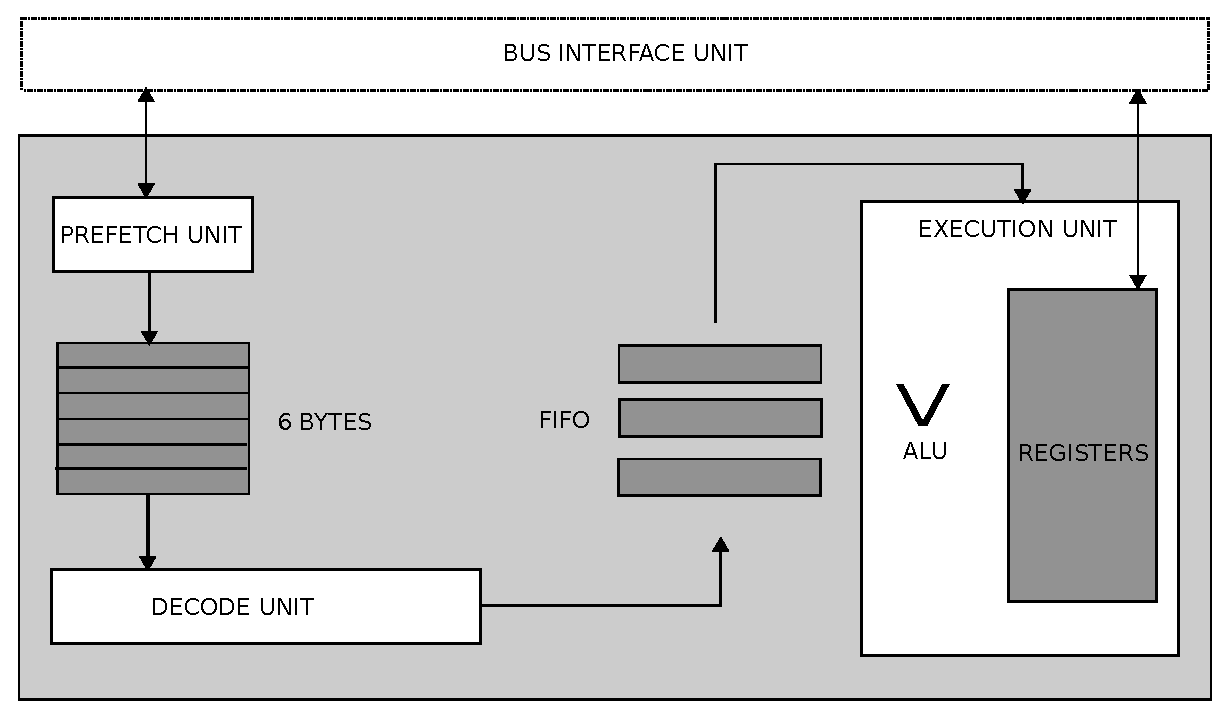
\includegraphics[width=\textwidth]{imgs/drawings/processing_unit.eps}
\end{figure}
\par
The three units in the execution group form a three stage pipeline: Prefetch, Decode, and Execute. The Prefetch Unit wakes up when the Execution unit is performing but not using the bus and fetches instructions in a 6-byte queue. The prefetcher is linear and cannot predict the result of a branch. As a result, a jump (\cw{JMP}) instruction triggers a flush of the entire pipeline. Instructions go down the pipeline and are decoded by the Decode Unit: the result of the decode operation is stored in a three-element FIFO where it is picked up by the Execution Unit.\\
\par

\begin{figure}[H]
\centering
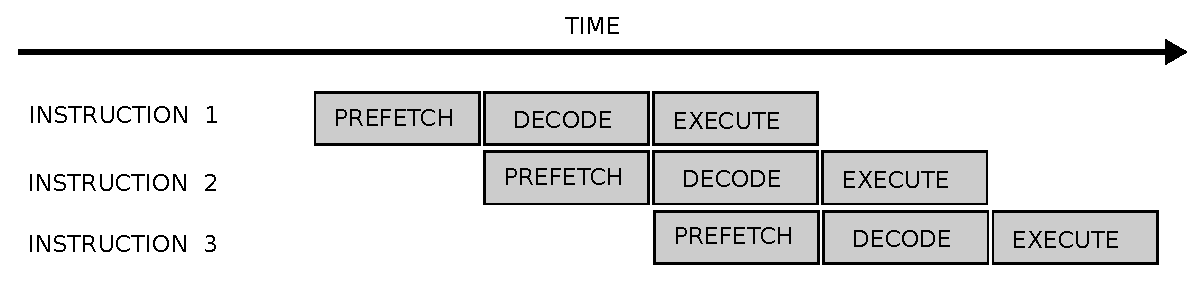
\includegraphics[width=\textwidth]{imgs/drawings/instruction_pipeline.eps}\\
\end{figure}
\par
\begin{figure}[H]
\centering

  \fullimage{Intel80286.png}
\caption{The Intel 286, 10mm by 10mm packing 134,000 transistors}
\end{figure}
\par
From a programming perspective, a 286 CPU can be summarized by the following elements:
\begin{itemize}
\item Arithmetic Logic Unit performing \cw{add}, \cw{sub}, \cw{mul} et cetera.
\item 14 registers:
\begin{itemize}
  \item 16-bit General Purpose Registers: AX, BX, CX, DX
  \item 16-bit Index Registers: SI, DI, BP, SP
  \item 16-bit Segment Registers: CS, DS, ES, SS
  \item 16-bit Status and Control Register
  \item 16-bit Program Counter: IP
\end{itemize}
\item A 24-bit address bus for up to 16MB of flat addressable RAM
\item Memory Management Unit
\end{itemize}
 \par

Despite its pipeline design, the 286 cannot do an operation in less than two cycles. Even a simple \cw{ADD reg, reg} or \cw{INC reg} takes two clocks. This is due to the absence of a SRAM on-chip cache and a slow decoding unit. Also have a look at multiplications which cost 24 cycles. So as a game developer you really want to avoid many multiplications during game runtime.\\
 \par
 

  \begin{figure}[H]
\centering  
\begin{tabularx}{\textwidth}{ X  Y }
  \toprule
  \textbf{Instruction type} &  \textbf{Clocks} \\
  \toprule 
   \cw{ADD reg8, reg8} & 2  \\
   \cw{INC reg8} & 2  \\
   \cw{IMUL reg16, reg16} & 24  \\
   \cw{IDIV reg16, reg16} & 28 \\
   \cw{MOV [reg16], reg16} & 5 \\
   \cw{OUT [reg16], reg16} & 3 \\
   \cw{IN [reg16], reg16} & 5 \\
  \toprule
\end{tabularx}
\caption{286 instruction costs\protect\footnotemark}
\end{figure}
\addtocounter{footnote}{-1}
\stepcounter{footnote}
\footnotetext{Intel 80286 programmer's reference manual - 1987.}


\subsection{16-bit Data alignment}
Compared to the Intel 8088, the 286 CPU contained a 16-bit external data bus where the 8088 only had a 8-bit bus. Thanks to its 16-bit bus, the 286 can access and write word-sized memory variables just as fast as byte-sized variables. There's a catch, however: That's only true for word-sized variables that start at even memory addresses. When the 286 is asked to perform a word-sized access starting at an odd memory address, it actually performs two separate accesses, each of which fetches 1 byte, just as the 8088 does for all word-sized accesses. In other words, the effective capacity of the 286's external data bus is halved when a word-sized access to an odd address is performed\footnote{See Michael Abrash's Graphics Programming Black Book Special Edition, chapter 11.}.\\

\begin{figure}[H]
\centering
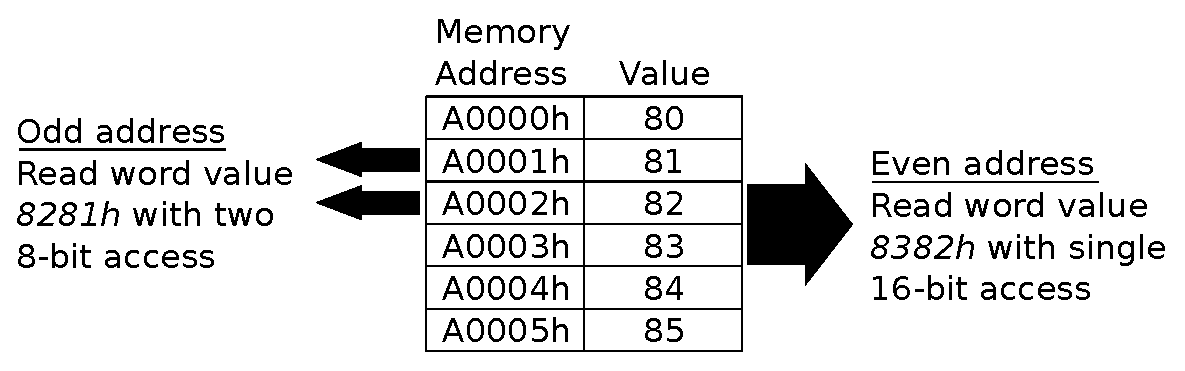
\includegraphics[width=\textwidth]{imgs/drawings/data_alignment.eps}\\
\end{figure}
\par

\par
The way to deal with the data alignment cycle-eater is straightforward: Don't perform word-sized accesses to odd addresses on the 286 if you can help it. This is not an issue for small memory operations, but it will harm performance when copying large memory blocks. 



\section{RAM}
The first CPUs in the Intel x86 family were designed in 1976. It was introduced at a time when the largest register in a CPU was only 16-bits long which meant it could address only 65,536 bytes (64 KiB\footnote{This book uses IEC notation where KiB is $2^{10}$ and KB is $10^3$.}) of memory, directly. As example both  the Apple II and the Commodore 64 both shipped with 64KiB which was enough to write and run amazing things.\\

\par
But everyone was hungry for a way to run much larger programs. Rather than create a CPU with larger register sizes, the designers at Intel decided to keep the 16-bit registers for their new 8086 and 8088 CPU and added a different way to access more memory: They expanded the instruction set, so programs could tell the CPU to group  two 16-bit registers together whenever they needed to refer to an absolute memory location beyond 64 KiB.\\

\subsection{Memory addressing}
If the designers had allowed the CPU to combine two registers into a high and low pair of 32-bits, it could have referenced up to 4 GiB of memory in a linear fashion. Keep in mind, however, this was at a time when many never dreamed we'd need a PC with more than 640 KiB of memory for user applications and data\footnote{We've often heard that Bill Gates said something to the effect: "640K of memory should be enough for anyone.". Though many of us no longer believe he ever said those exact words, he did, however, during a video interview with David Allison in 1993 for the National Museum of American History, Smithsonian Institution, say: "I laid out memory so the bottom 640KiB was general purpose RAM and the upper 384KiB I reserved for video and ROM, and things like that."}. So, instead of dealing with whatever problems a linear addressing scheme of 32-bits would have produced, they created the Segment:Offset scheme 
which allows a CPU to effectively address about 1 MiB\footnote{This book uses IEC notation where MiB is $2^{20}$ and MB is $10^6$.} of memory. The Segment:Offset schema combines two 16-bit registers, one designating a segment and the other an offset within that segment.
\\

\par
\begin{figure}[H]
\centering
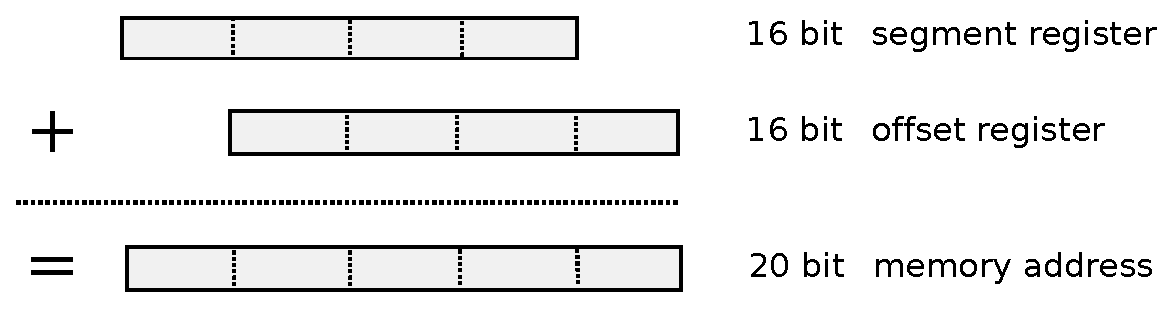
\includegraphics[width=\textwidth]{imgs/drawings/register_combination_20_bits_address.eps}
\caption{How registers are combined to address memory.}
\label{fig:register_comb_to_20_bits}
\end{figure}
\par

To support this architecture, the CPU keeps track of four different segments. Each of these segments has its own purpose and segment register:
\begin{itemize}
  \item CS segment register, where the machine instructions resides.
  \item DS segment register, where the data resides.
  \item SS segment register, where the stack resides.
  \item ES segment register, which is used as extra data segment.
\end{itemize}

\par
In C-language a memory address can be accessed directly using pointers. A pointer is a variable that stores the memory address of another variable as its value. There are two kinds of pointers: \cw{near} and \cw{far}. \\

\par
A \cw{near} pointer refers to a function or data object that is within the current segment. It is 16 bits long and contains an offset into the current data segment if it's a data pointer, or into the current code segment if it's a function pointer. A \cw{far} pointer refers to a function or data that is in a different segment than the current, default one. It is 32 bits long and contains a segment and offset, which identifies the location where the code or data is stored. \\

\par
Accessing code or data with a \cw{near} reference is much quicker than accessing it with a \cw{far} pointer. When you use a \cw{far} reference, your program must first find the segment and then find the code or data within that segment. When you use a \cw{near} reference, your program only needs to find the code or data via the offset. For a faster program, one should make as many \cw{near} references as possible. The downside of using \cw{near} pointers only is that it can handle not more than 64KiB of memory for the program or data.\\


Note that a \cw{far} pointer only increments the offset, not the segment. If you iterate on a data array larger than 64KiB there will be no overflow handling, so you will be able to handle only 64KiB of memory.\\

\par
\begin{minipage}{\textwidth}
 \lstinputlisting[language=C]{code/far_pointer.c}\par
 \end{minipage}\\
\par
Will output:\\
\par
\begin{minipage}{\textwidth}
 \lstinputlisting[language=C]{code/far_pointer_out.c}\par
 \end{minipage}\\

\par
You could use yet another type of pointer named \cw{huge} to make pointer arithmetic work beyond 64KiB. \\
\par
\begin{minipage}{\textwidth}
 \lstinputlisting[language=C]{code/huge_pointer.c}\par
 \end{minipage}\\
\par
Will output the address:\\
\par
\begin{minipage}{\textwidth}
 \lstinputlisting[language=C]{code/huge_pointer_out.c}\par
 \end{minipage}\\
\par

The \cw{huge} pointer is based on the absolute (or lineair) 20-bit memory location and Segment:Offset normalized address. The absolute memory address can be calculated by\\

\par
\begin{minipage}{\textwidth}
\lstinputlisting[ language={[x86masm]Assembler}]{code/segment_offset}
\end{minipage}\\

\par
For example the absolute address of \cw{A000:002F} is \cw{A0000h} + \cw{002Fh} = \cw{A002Fh}. By confining the offset to just the hexadecimal values \cw{0h} through \cw{Fh}, we have a unique way to reference all Segment:Offset memory pair locations. To convert an arbitrary Segment:Offset pair into a normalized address is a two-step process that's quite easy for an assembly programmer:\\

\begin{enumerate}
  \item Convert the Segment:Offset pair into a single absolute address.
  \item Then simply insert the colon (:) between the last two hex digits and add three zeros before the last hex digit.
\end{enumerate}

For example, the normalized address for \cw{A000:002F} is \cw{A002:000F}. A \cw{huge} pointer is normalized when pointer arithmetic is performed on it. \\
\par
\begin{minipage}{\textwidth}
 \lstinputlisting[language=C]{code/huge_pointer_normalized.c}\par
 \end{minipage}\\
\par
Will output:\\
\par
\begin{minipage}{\textwidth}
 \lstinputlisting[language=C]{code/huge_pointer_norm_out.c}\par
 \end{minipage}\\
\par



\trivia{Since the normalized form will always have three leading zero bytes in its offset, programmers often write it with just the digit that counts: \cw{AFFF:F}}\\

\par
A \cw{huge} reference is even slower than the \cw{far} reference as it comes with additional overhead to update the segment and address normalization after every arithmetic manipulation. So, most programmers avoided the \cw{huge} pointer, unless really needed.\\

\subsection{80286 Real and Protected mode}
By 1986, hardware had gotten cheaper and Intel made a departure from the old architecture
with its 286. This new CPU could be put in what is called "protected mode" featuring
a 24-bit-wide address bus for up to 16 MiB of flat RAM protectable with a MMU\footnote{Memory Management Unit}. To make sure old programs could still run, the 286 processor could be put in "real mode" which replicates how the Intel 8086 and 8088 operated: 16-bit registers, 20-bit address bus giving 1MiB addressable RAM with segmented addressing.\\

\par
For compatibility reasons all PCs have to start in real mode. You may assume that programmers
of the late 80s promptly switched the CPU to protected mode to unleash the full
potential of the machines and ditch the 20-year-old real mode. It would have worked out if the operating system had been able to run in protected mode.
However, in the name of backward compatibility, Microsoft's DOS could only handle real
mode which effectively locked developers into 16-bit programming\footnote{16-bit programming and memory managers were covered in Game Engine Black Book: Wolfenstein 3D.}.\\


\par
  With protected mode unavailable, 1990 developers programmed like it was 1976: with a 20-bit-wide address bus offering only 1MiB of addressable RAM. Regardless how much memory was installed on the machine, only 1MiB could be addressed. The memory layout for the real mode is as follows:
\begin{itemize}
\item From 00000h to 003FFh : the Interrupt Vector Table.
\item From 00400h to 004FFh : BIOS data.
\item From 00500h to 005FFh : command.com+io.sys.
\item From 00600h to 9FFFFh : Usable by a program (about 620KiB in the best case). 
\item From A0000h to FFFFFh : UMA (Upper Memory Area): Reserved to BIOS ROM, video card and sound card mapped I/O.
\end{itemize}


\bigskip
Out of the original 1024KiB, only 640KiB (called Conventional Memory) was accessible to a program. 384KiB was reserved for the UMA and every single driver installed (\codeword{.SYS} and \codeword{.COM}) took away from the remaining 640KiB.\\

\par
\begin{figure}[H]
\centering
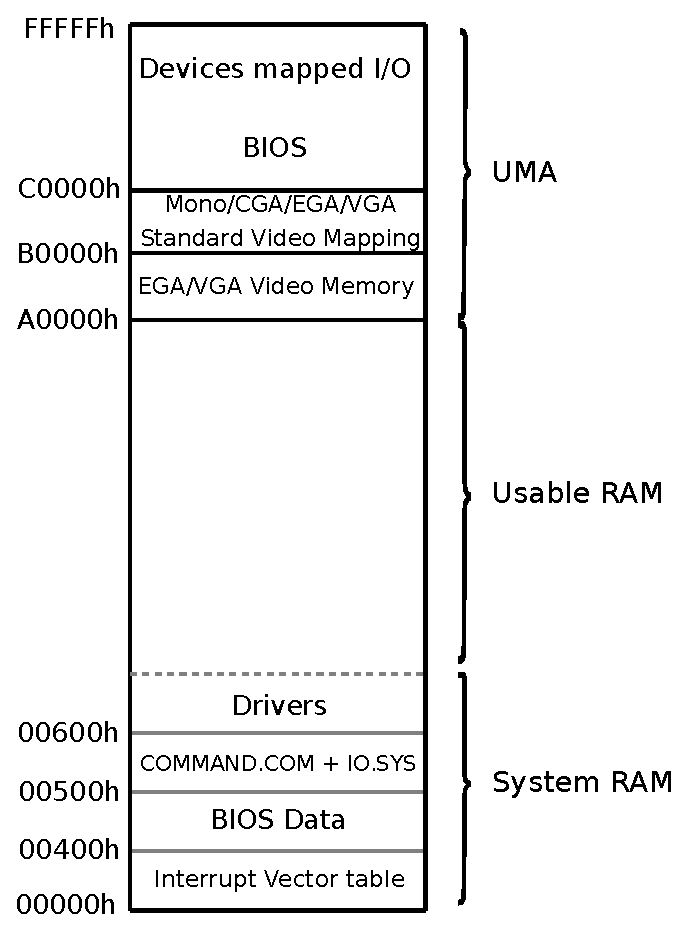
\includegraphics[width=0.8\textwidth]{imgs/drawings/real_mode_v2.eps}
\caption{First 1MiB of RAM layout.}
\label{fig:fp_internals}
\end{figure}
\pagebreak

\subsection{Real mode: Memory models}
The x86 real mode provided different memory segment layouts which are called \textit{memory models}. Each memory model controls how the segment registers are organized as well as defining the default pointer type to \cw{near} or \cw{far}. Functions and pointers within a given program default to \cw{near} or \cw{far}, depending on the memory model you select. If the function or data pointer is \cw{near}, it is automatically associated with either the CS or DS register.\\

\par
In total six different memory models are defined, making trade-offs between minimum system requirements, maximizing code efficiency, and gaining access to every available memory location\footnote{See Borland C++ 3.1 Programmer's guide, section DOS Memory management.}. 

\begin{figure}[H]
\renewcommand{\arraystretch}{1.2}
\centering
\begin{tabularx}{\textwidth}{|X|X|X|X|X|>{\hsize=.3\textwidth}Y|} \hline
  &  \multicolumn{2}{c|}{\textbf{Default pointer type}} & \multicolumn{2}{c|}{\textbf{Size}} &  \\ \cline{2-5}
 \textbf{Model}   & \textbf{Code} & \textbf{Data} & \textbf{Code} & \textbf{Data} & \textbf{Definition} \\ \hline
 Tiny & near & near & \multicolumn{2}{c|}{<64KiB} & CS=DS=SS \\ \hline
 Small & near & near & <64KiB & <64KiB & DS=SS \\ \hline
 Medium & far & near & >64KiB & >64KiB & DS=SS, multiple CS \\ \hline
 Compact & near & fear & <64KiB & >64KiB & DS only global/static data\\ \hline
 Large & far & far & >64KiB & >64KiB & multiple CS,  DS only global/static data \\ \hline
 Huge & far & far & >64KiB & >64KiB & multiple CS and DS, DS only global/static data \\ \hline
 

\end{tabularx}\\
\end{figure}

As memory is scarce and every CPU cycle counts, a game developer needed a good understanding of each memory model and each compications. Each application consists out of the following building blocks:
\begin{itemize}
  \item code block where all C-functions and routines reside.
  \item static data block which contains all global and static variables. 
  \item the stack, which contains mainly local and temporarily data.
  \item the heap, which contains dynamic allocated memory via \cw{malloc()} function
\end{itemize}

\pagebreak
Let's start to understand how the first, tiny memory model, is organized. All three segment registers, CS, DS and SS, point to the same memory location. The first part of the segment is used for all machine instructions, followed by the static and global data. The heap is starting directly after the static and global data and grows upwards. Finally, the stack is starting at the opposite side of the segment and is growing downwards. Both heap and stack can grow/shrink dynamically during program execution. When both the heap and stack continue to grow, ultimately they collide which results in an unwanted \cw{"memory error"}.\\

\begin{figure}[H]
\centering
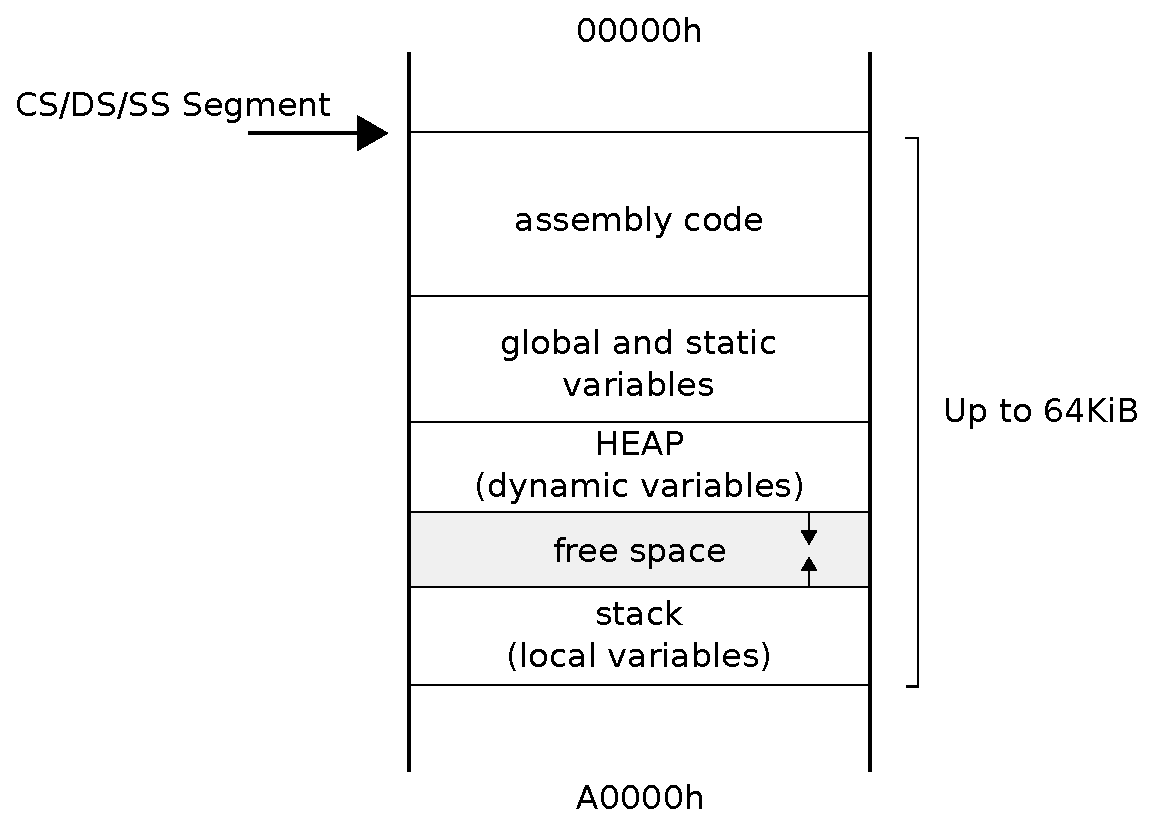
\includegraphics[width=0.7\textwidth]{imgs/drawings/tiny_mm.eps}
\caption{Tiny memory model.}
\label{fig:mm_tiny}
\end{figure}
\par

All function and data pointers are accessed via a \cw{near} reference, which means they are automatically associated with either the CS or DS segment register. Since only \cw{near} references are used the program execution is very efficient, but there is also a downside: The instructions, data and stack all share the same segment of maximum 64KiB.\\

\par
The next model, the small memory model, separates the instructions from the data, each having their own 64KiB segment. The code segment has a maximum size of 64KiB for instructions, and the data, stack and heap share a separated 64KiB segment. The code remains executed efficient as all functions and data pointers are accessible via a \cw{near} reference.\\

\begin{figure}[H]
\centering
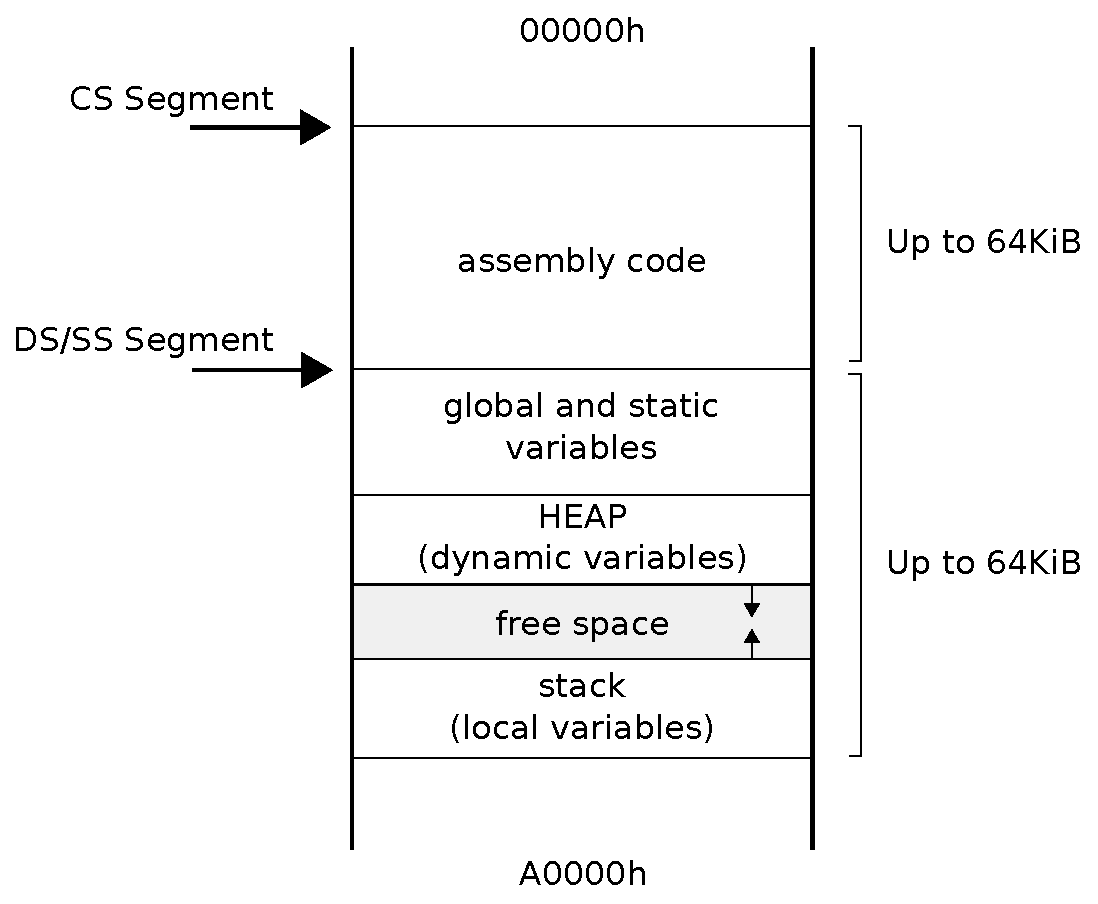
\includegraphics[width=0.7\textwidth]{imgs/drawings/small_mm.eps}
\caption{Small memory model, code and data each have 64KiB.}
\label{fig:mm_small}
\end{figure}
\par

If the function code requires more than 64KiB, the medium memory model is an outcome. Now each C source file has its own code segment.  A table with all code segment references is maintained and the CS register points to only one segment at the time. There is no default CS segment, and functions must be reached using a \cw{far} reference. The code is executed less efficient compared to the tiny and small memory models.\\

\trivia{When you compile a source file, the resulting code for that file cannot be greater than 64KiB, since it must all fit inside one code segment. If the source file is too big to fit into one (64KiB) code segment, the programmer must break it up into different source code files, compile each file separately.}\\

\begin{figure}[H]
\centering
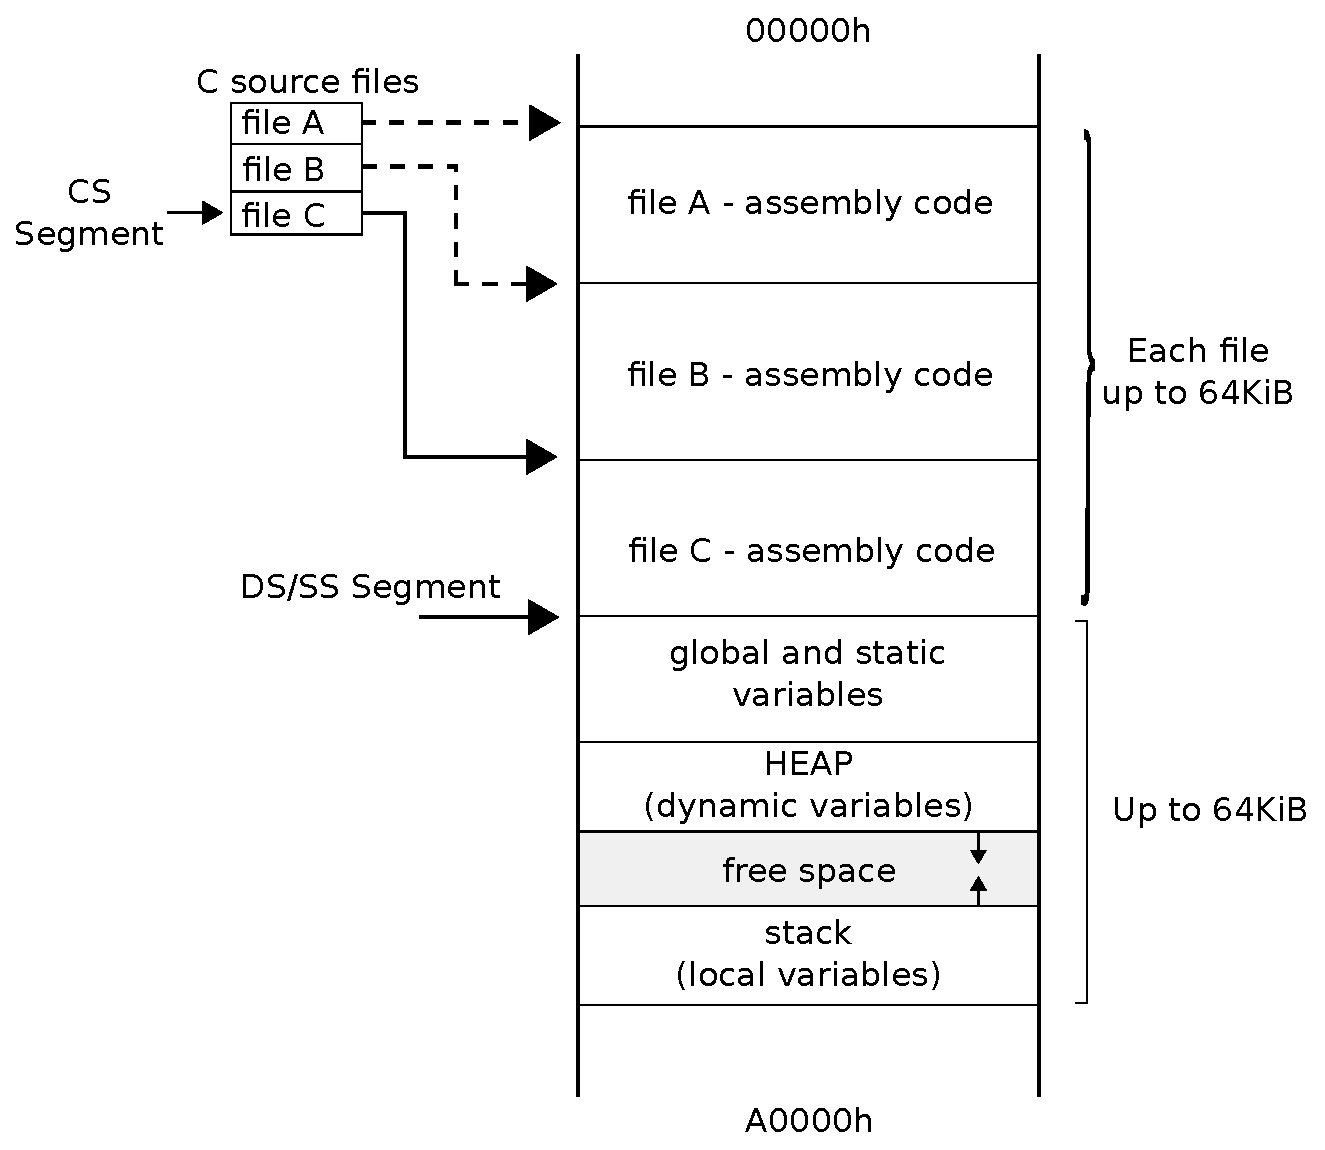
\includegraphics[width=0.9\textwidth]{imgs/drawings/medium_mm.eps}
\caption{Medium memory model, code can be larger than 64KiB.}
\label{fig:mm_medium}
\end{figure}
\par

\par
Most games rely on dynamic memory allocation to load data like graphics and levels. Game data is loaded from disk when starting a level, so the size is not known when the game is initially executed. Loading all data for a level often requires a large portion of dynamic memory. As the heap is using the same default DS segment as global data and the stack, it most likely won't fit and results in a \cw{out of memory} error. \\

\par
Luckily, in both the small and medium model, the memory between the stack and \cw{A0000h} is available to the game developer. It is called the \textit{farheap}, and can be allocated using the \cw{farmalloc()} function. The memory can only be accessed using a \cw{far} or \cw{huge} pointer reference. 

\begin{figure}[H]
\centering
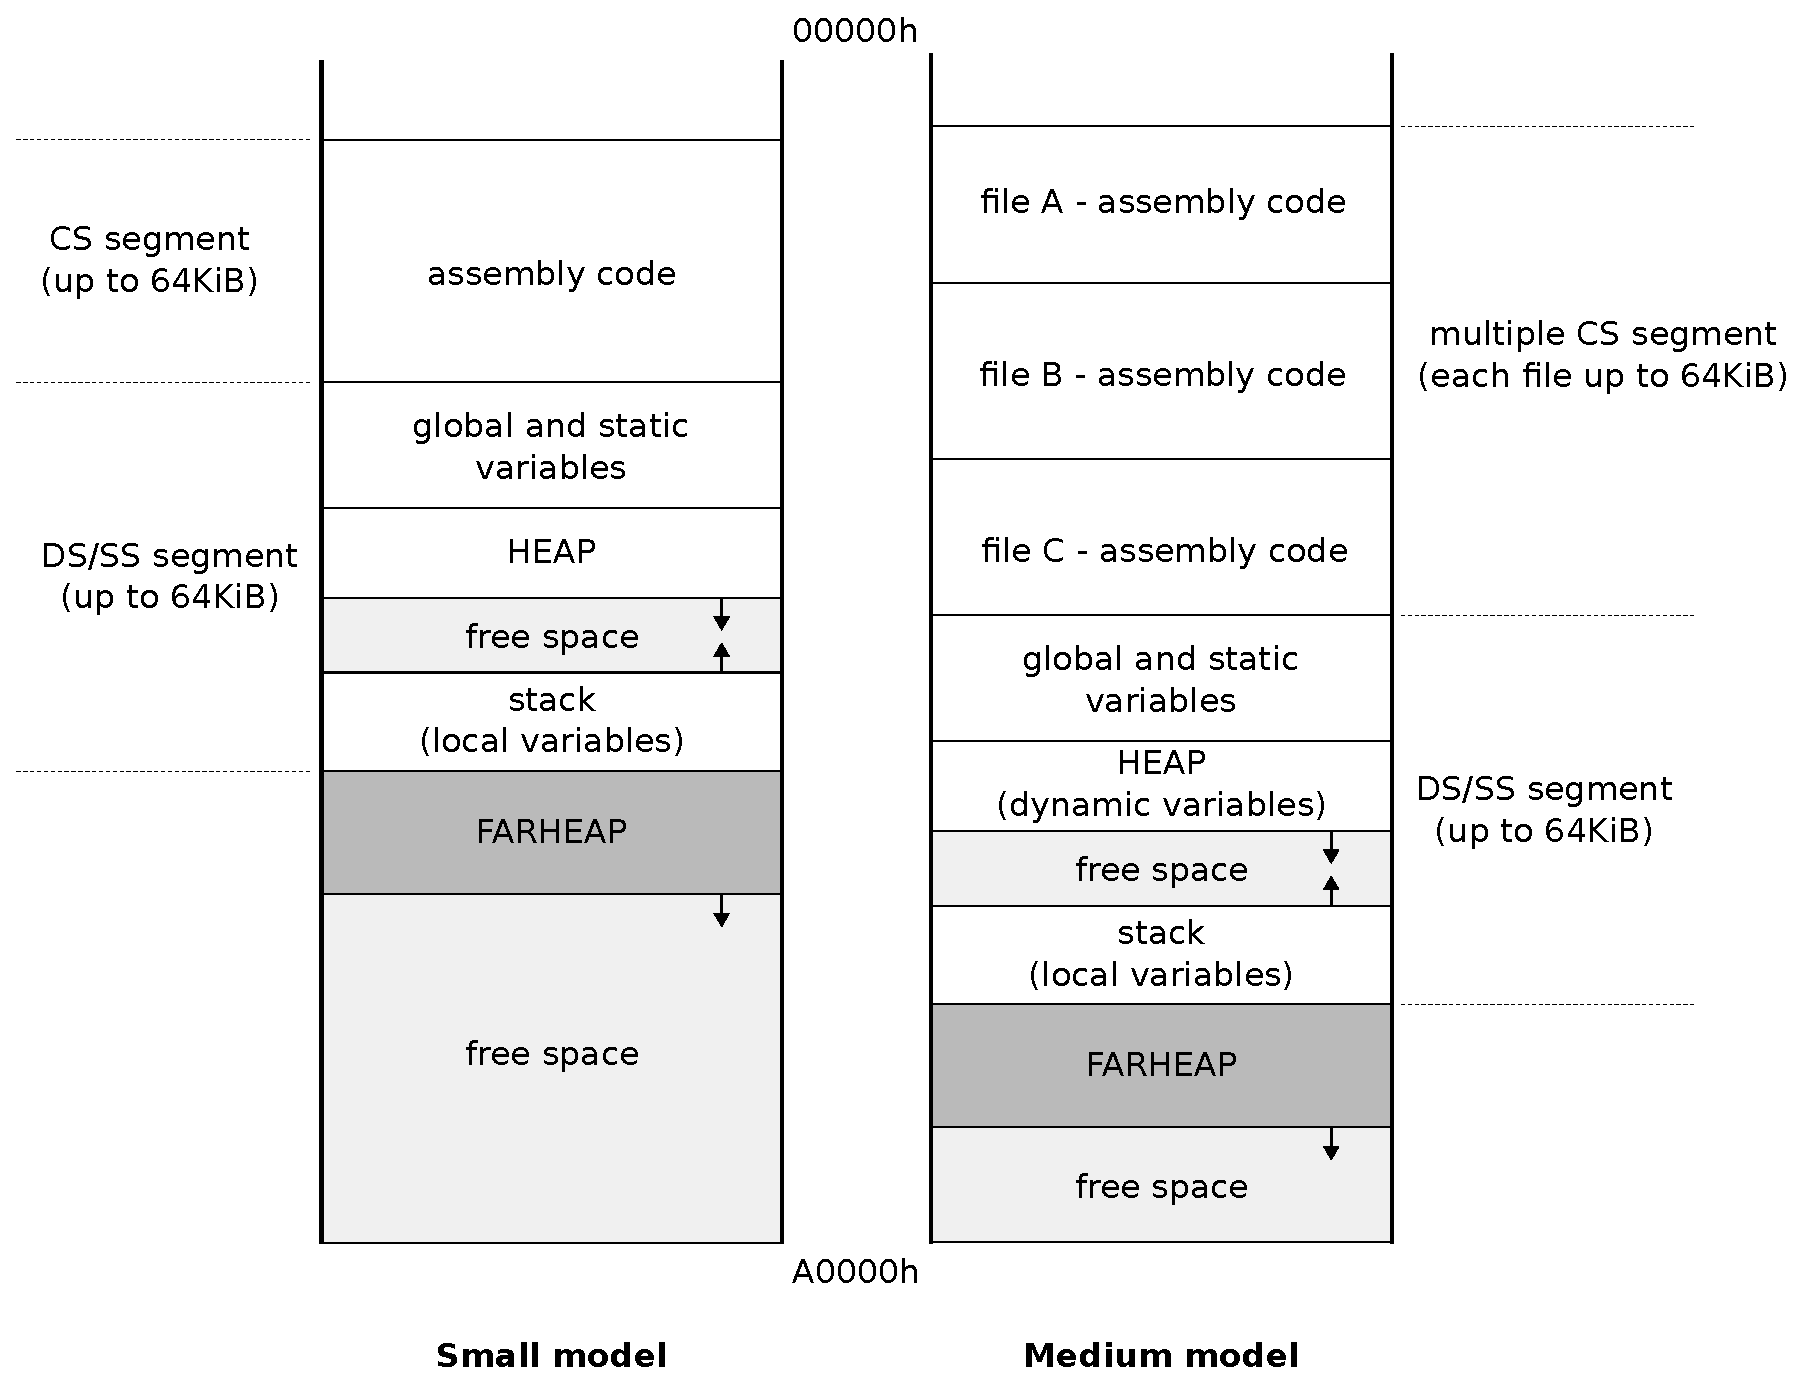
\includegraphics[width=1.0\textwidth]{imgs/drawings/farheap_mm.eps}
\caption{farheap memory between stack and \cw{A0000}.}
\label{fig:mm_farheap}
\end{figure}
\par

The opposite of the medium model is the compact model. Here the total function code is smaller than 64KiB, but data can exceed 64KiB. Both the large and huge model can deal with function code and data larger than 64KiB, but are slow in execution as they cannot use \cw{near} references.\\  

\par
Commander Keen is, like many games during that period, making ise of the medium memory model. It provides the best trade-off between code size (more than 64Kib), efficient access to global data using \cw{near} pointers and sufficient memory for dynamic allocation. \\

<<PICTURE OF BORLAND>>\\

\pagebreak


\section{Video}

PCs were connected to CRT monitors: big, heavy, small diagonal, cathode ray-based, curved-surface screens. Most had a 14" diagonal with a 4:3 aspect ratio.\\
\par


\begin{figure}[H]
\centering
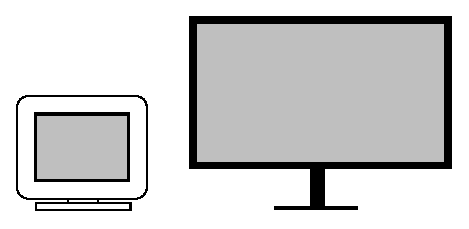
\includegraphics[width=\textwidth]{imgs/drawings/crt_lcd.eps}
\caption{CRT (left) vs LCD (right)}
\label{fig:lcd_vs_crt}
\end{figure}
\par
  To give you an idea of the size and resolution, figure \ref{fig:lcd_vs_crt} shows a comparison between a 14" CRT from 1990 (capable of a resolution of 640x200) and a 30" Apple Cinema Display from 2014 (capable of a resolution of 2560x1600).\\
  \par
\trivia{Despite their difference of capabilities, both monitors are the same weight: 27.5 pounds (12 kg).}
\\

\subsection{CRT Monitor}
All standard PC monitors use a raster-scan display to create the image.
In a raster-scan display, the position of the electron beam is continually sweeping across the surface of the tube. The tube's surface is coated with phosphors that glow when struck by electrons (and for a short time thereafter), and, of course, the beam may be turned on in order to light a phosphor or off to leave it black.\\
\par

The electron beam scans the phosphor-coated screen from left to right and
top to bottom. The period during which the beams return to the left is known as
the horizontal retrace. During most of the retrace, the guns must be turned off
to prevent writing in the active display area (the area which contains the actual
character and/or graphics data); this is known as horizontal blanking.\\

\par
The area immediately surrounding the display area, in which the beam may be turned on
during the retrace interval, is called the overscan (or border). The active display
area is the portion of the screen that contains characters and/or graphics. These
components of the scan are shown in simplified form in Figure \ref{fig:monitor}.\\

\begin{figure}[H]
\centering
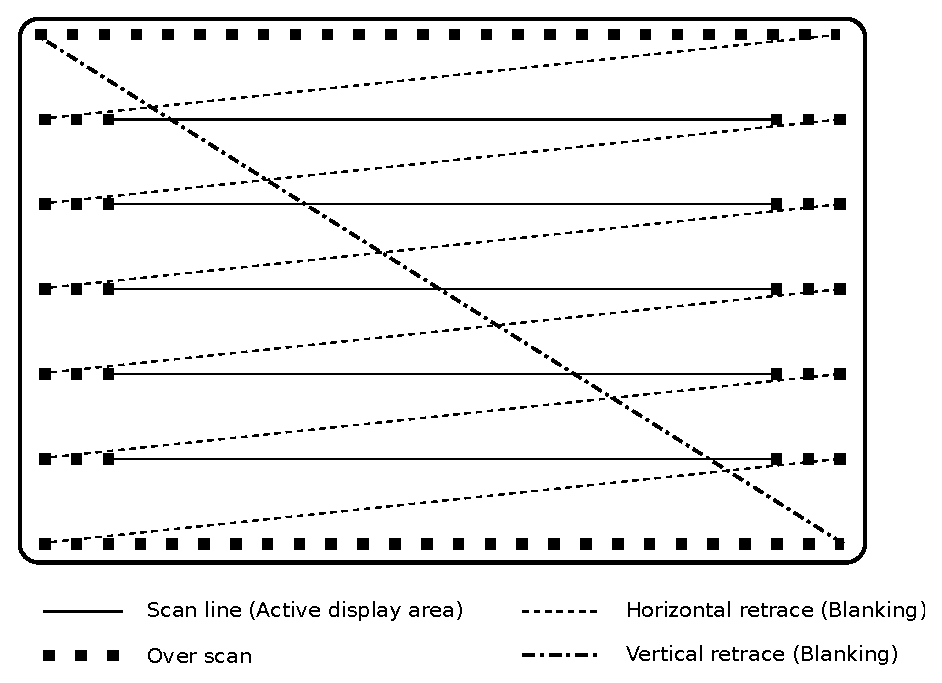
\includegraphics[width=\textwidth]{imgs/drawings/monitor.eps}
\caption{Simplified CRT monitor scan.}
\label{fig:monitor}
\end{figure}

\par
After a horizontal scan has been completed, the beam is moved to the next
line during the horizontal retrace. This sequence continues until the last line, at which point the vertical retrace begins. The vertical retrace is similar to the horizontal retrace; the electron beam may be enabled through a small overscan area and then turned off (vertical blanking) as the beam returns to the top left comer of the screen.\\

\par
If the vertical refresh is too slow, the display will flicker. Most people can detect flicker when the refresh rate drops below 60 Hz, and thus most displays use vertical refresh frequencies of about 60Hz (EGA) to 70Hz (VGA). 



  \subsection{History of Video Adapters}

The Monochrome Display Adapter (\codeword{MDA}) was released in 1981 with the IBM PC 5150. It offered two colors, allowing 80 columns by 25 lines of text.  While not great, it was standard on every PC. Many other systems followed over the years, each of them preserving backward compatibility.

\bigskip
 \begin{figure}[H]
\centering  
\begin{tabularx}{\textwidth}{ l X l Y }
  \toprule
  \textbf{Name} &  \textbf{Year Released} & \textbf{Memory} & \textbf{Max Resolution}\\
  \toprule \codeword{MDA}
   (\textbf{M}onochrome
   \textbf{D}isplay
   \textbf{A}dapter) & 1981 & 4KiB & 80x25\footnotemark 
   \\ \codeword{Hercules} & 1982 & 64KiB & 720x348
   \\ \codeword{CGA}
   (\textbf{C}olor
   \textbf{G}raphics
   \textbf{A}dapter) & 1981 & 16KiB & 640x200
    \\ \codeword{EGA}
   (\textbf{E}nhanced
   \textbf{G}raphics
   \textbf{A}dapter) & 1985 & 64KiB & 640x350
   \\ \codeword{VGA}
   (\textbf{V}ideo
   \textbf{G}raphics
   \textbf{A}rray)  & 1987 & 256KiB & 640x480
    \\
  \toprule
\end{tabularx}
\caption{Video interface history.}\label{fig:vga_history}
   
\end{figure}
\addtocounter{footnote}{-1}
\stepcounter{footnote}
\footnotetext{Text mode only.}


Each iteration added new features and by 1990 the predominant graphic system was EGA, although the VGA system was rapidly becoming the new standard. All video cards installed on PCs had to follow the standard set by IBM. The universality of that system was a double-edged sword. While developers had to program for only one graphic system, there was no escaping its shortcomings.\\


\subsection{Introduction of EGA Video Card}

IBM introduced the Enhanced Graphics Adapter (EGA) in 1985 as the successor of CGA. The standard card was shipped with only 64KiB video memory, but it had the option to expand the memory using the onboard graphics memory expansion card.
Figure \ref{fig:ibm_ega_card} shows the original IBM EGA card, a clunky beast full of discrete components. The memory consists out of TMS4416 RAM, a common memory chip for (home) computers around that period. Each chip contains 16KiB of 4-bits memory, so one needs two chips to end up having 16KiB of 8-bit memory and eight chips for 64KiB of 8-bit memory. \\

\trivia{Texas Instruments introduced the first 16KiB by 4-bits as TMS4416 in 1980\footnote{https://pdf1.alldatasheet.com/datasheet-pdf/view/103706/TI/TMS4416.html}. Still it took until 1983-84 until they became widely available and lower priced than four TMS4116 chips (16KiB by 1-bit). However, at that time 64 KiB RAM was the way to go for new designs. Computers with only 16 KiB as base memory - and that's where TMS4416 would have been a cost saver - were already on the way out.}\\


\begin{figure}[H]
  \centering 
  \includegraphics[width=1.3\textwidth, angle =90 ]{screenshots_300dpi/hardware/ibm_ega_card.png} 
  \caption{Original IBM EGA card}
  \label{fig:ibm_ega_card}
\end{figure}

\par
To add additional video memory to the IBM EGA card a Graphics Memory Expansion Card could be purchased. By default only the bottom row of memory was populated with chips, expanding the total EGA video memory to 128KiB. The expansion card provided DIP (dual in-line package) sockets for further memory expansion. Populating the DIP sockets with a Graphics Memory Module Kit adds two additional rows of 64KiB, bringing the EGA memory to its maximum of 256KiB. \\


\begin{figure}[H]
  \centering 
  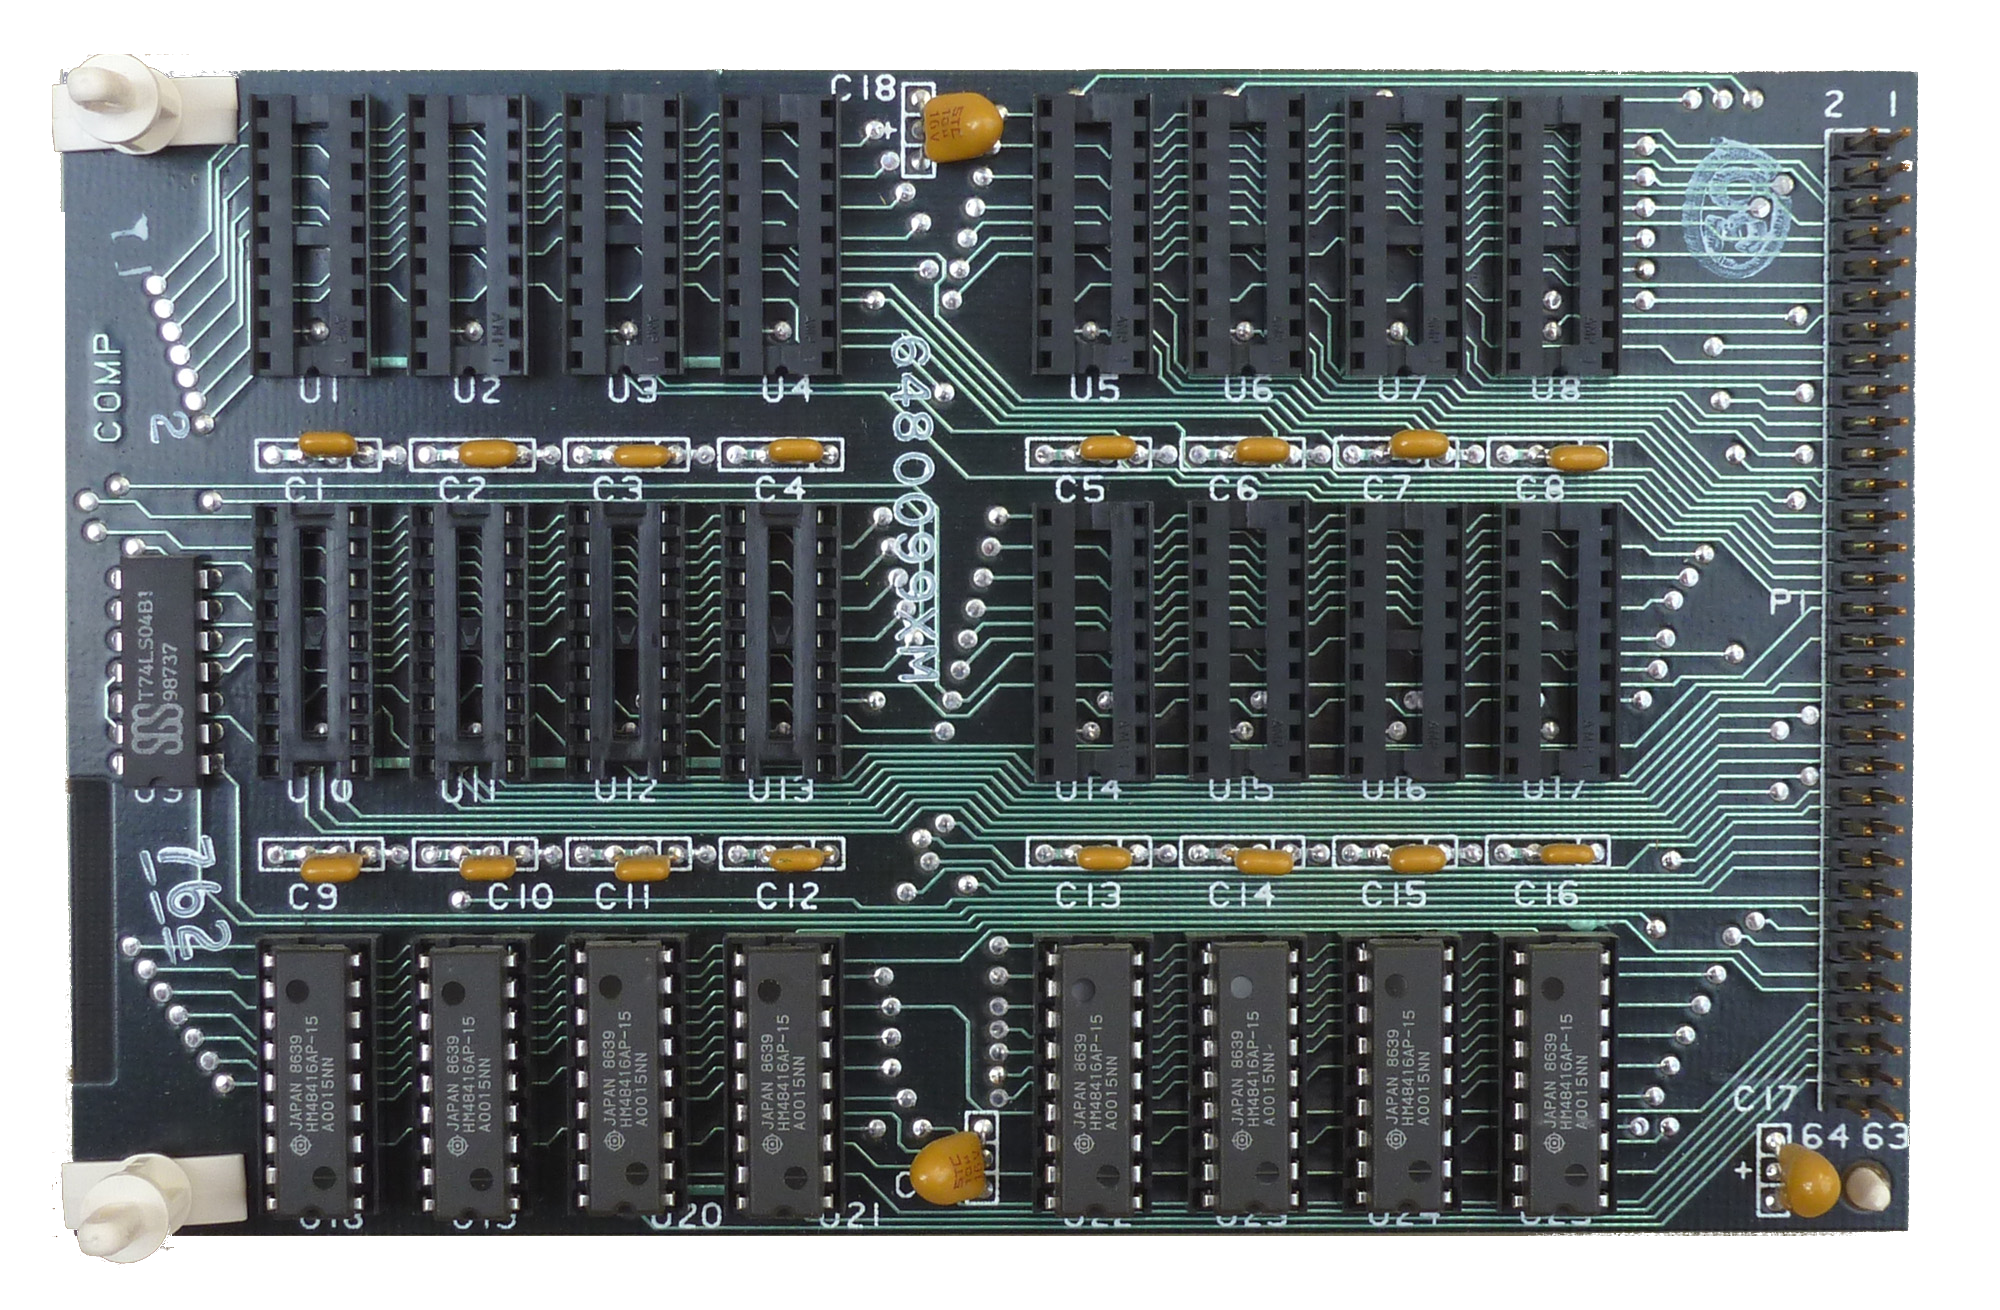
\includegraphics[width=1.0\textwidth]{screenshots_300dpi/hardware/ibm_ega_graphics_memory_expansion_card.png} 
  \caption{EGA Graphics Memory Expansion Card, bottom row populated with chips.}
  \label{fig:ibm_ega_card}
\end{figure}






\par
The EGA clones that started coming along in 1986-87 were based on integrated chipsets, and the vast majority of them came with the maximum of 256KiB on board. When Commander Keen came out, the headcount of EGA cards with less than 256KiB would've been practically negligible\footnote{PC Tech Journal Oct 1986 (page 82-83) and PC Tech Journal Nov 1986 (page 148-149)}.\\

\par
Below an ATI EGA Wonder 800 (8-bit ISA). The eight chips on the left of the card form the VRAM where the framebuffers are stored. 

\begin{figure}[H] 
  \centering 
  \scaledimage{0.9}{hardware/EGA-ATI-800.png} 
  
\end{figure}
\par
\pagebreak




\subsection{EGA Architecture}

EGA can be summarized as three major systems made of input, storage, and output:
\begin{itemize}
\item The Graphic Controller and Sequence Controller controlling how EGA RAM is accessed (the CPU-VRAM interface)
\item The framebuffer (the VRAM) made of four memory banks with 64KiB (rather than one bank of 256KiB).  
\item The CRT Controller and the Attribute Controller taking care of converting the palette-indexed framebuffer to RGB and then to digital TTL\footnote{Transistor Transistor Logic} signal for display
\end{itemize}

\par
\trivia{In the 1980's integrated video DACs\footnote{Digital to Analog Converter} were expensive and difficult to embed into custom chips. Most home computers with RGB output used TTL for digital output. With the introduction of VGA the DAC became the standard}.\\

The most surprising part of the architecture is obviously the framebuffer. Why have four small fragmented banks instead of one big linear one?\\
\par
The main reason was RAM latency and the need for minimum bandwidth. A CRT running at 60Hz and displaying 640x350 in 16 colors needs a pixel every $\frac{1}{640*350*60}=74$ nanosecond. At this resolution, one pixel is encoded with 4 bits. Each nibble is translated to a RGB color via the TTL. So that means it requires one byte every 148 nano-seconds.\\
\par
 Unfortunately, RAM access latency was 200ns - not nearly fast enough\footnote{Computer Graphics: Principles and Practice 2nd Edition, page 168.} to refresh the screen at 60hz, so the TTL would starve. If latency could not be reduced, the throughput could still be improved by reading from four banks at a time. Reading in parallel gave an amortized RAM latency of 200/4 = 50ns, which was fast enough.\\
\par
Keep in mind that this architecture reduced the penalty of read operations, but plotting a pixel in the framebuffer with a write operation was still slow. Writing to the VRAM as little as possible was crucial to maintaining a decent framerate. 


\begin{figure}[H]
\centering
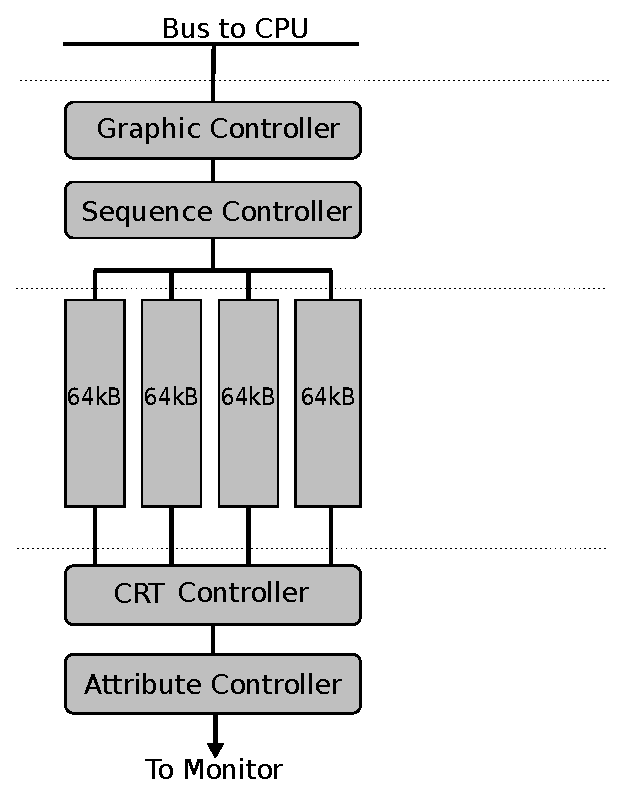
\includegraphics[width=0.9\textwidth]{imgs/drawings/ega.eps}
\caption{EGA Architecture.}
\label{fig:vga_arch}
\end{figure}




\subsection{EGA Planar Madness}
\label{section:EGA_Planar_Madness}

Four memory banks grant enough throughput to reach high resolutions at 60Hz. This type of architecture is called "planar". Each plane is like a black-and-white image that stores information about a single color. For EGA there are 4 planes, where combining one bit from each plane results in a color index. This color index is then via the attribute controller translated into a color to the screen. This layout is better explained with a drawing.\\

\par
To write the color of the first pixel, a developer has to write the first bit of the first byte in plane 0, the second in plane 1, the third in plane 2 and the fourth in plane 3. The CRT Controller then reads 4 bytes at a time (one from each plane) and converts them via the Attribute Controller into 8 pixels on screen. \\


\begin{figure}[H]
\centering
 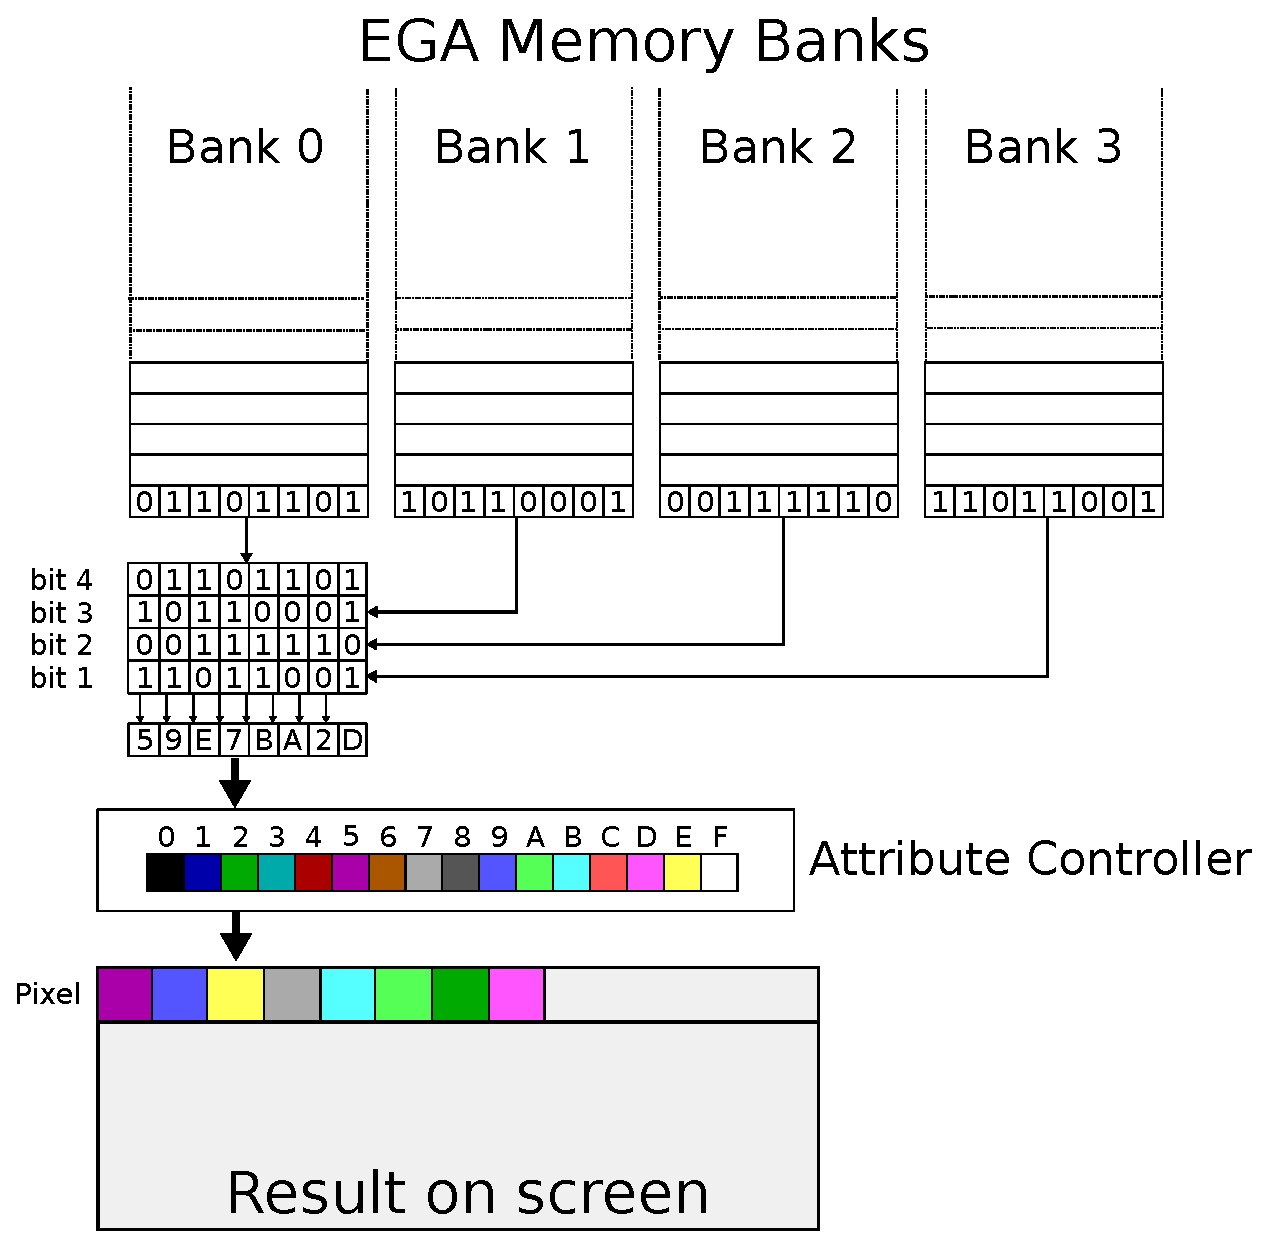
\includegraphics[width=1.0\textwidth]{imgs/drawings/mode0Dh.eps}
\caption{EGA mode 0Dh, how bank layout appears on screen.}
\label{fig:ega_bank_layout}
\end{figure}
 


\subsection{EGA Modes}
In order to configure this mess of planes and the controllers, 50 poorly documented internal registers must be set. Needless to say few programmers dove into the internals of the EGA.\\
\par
  Figure \ref{fig:vga_arch}, which described the architecture, was actually deceptively simplified. Figure \ref{fig:ibm_ega} shows how IBM's reference documentation explained the EGA. The maze of wire showcases well the actual complexity of the system.\\
 \par
 \vspace{10pt}
 \begin{figure}[H]
\centering
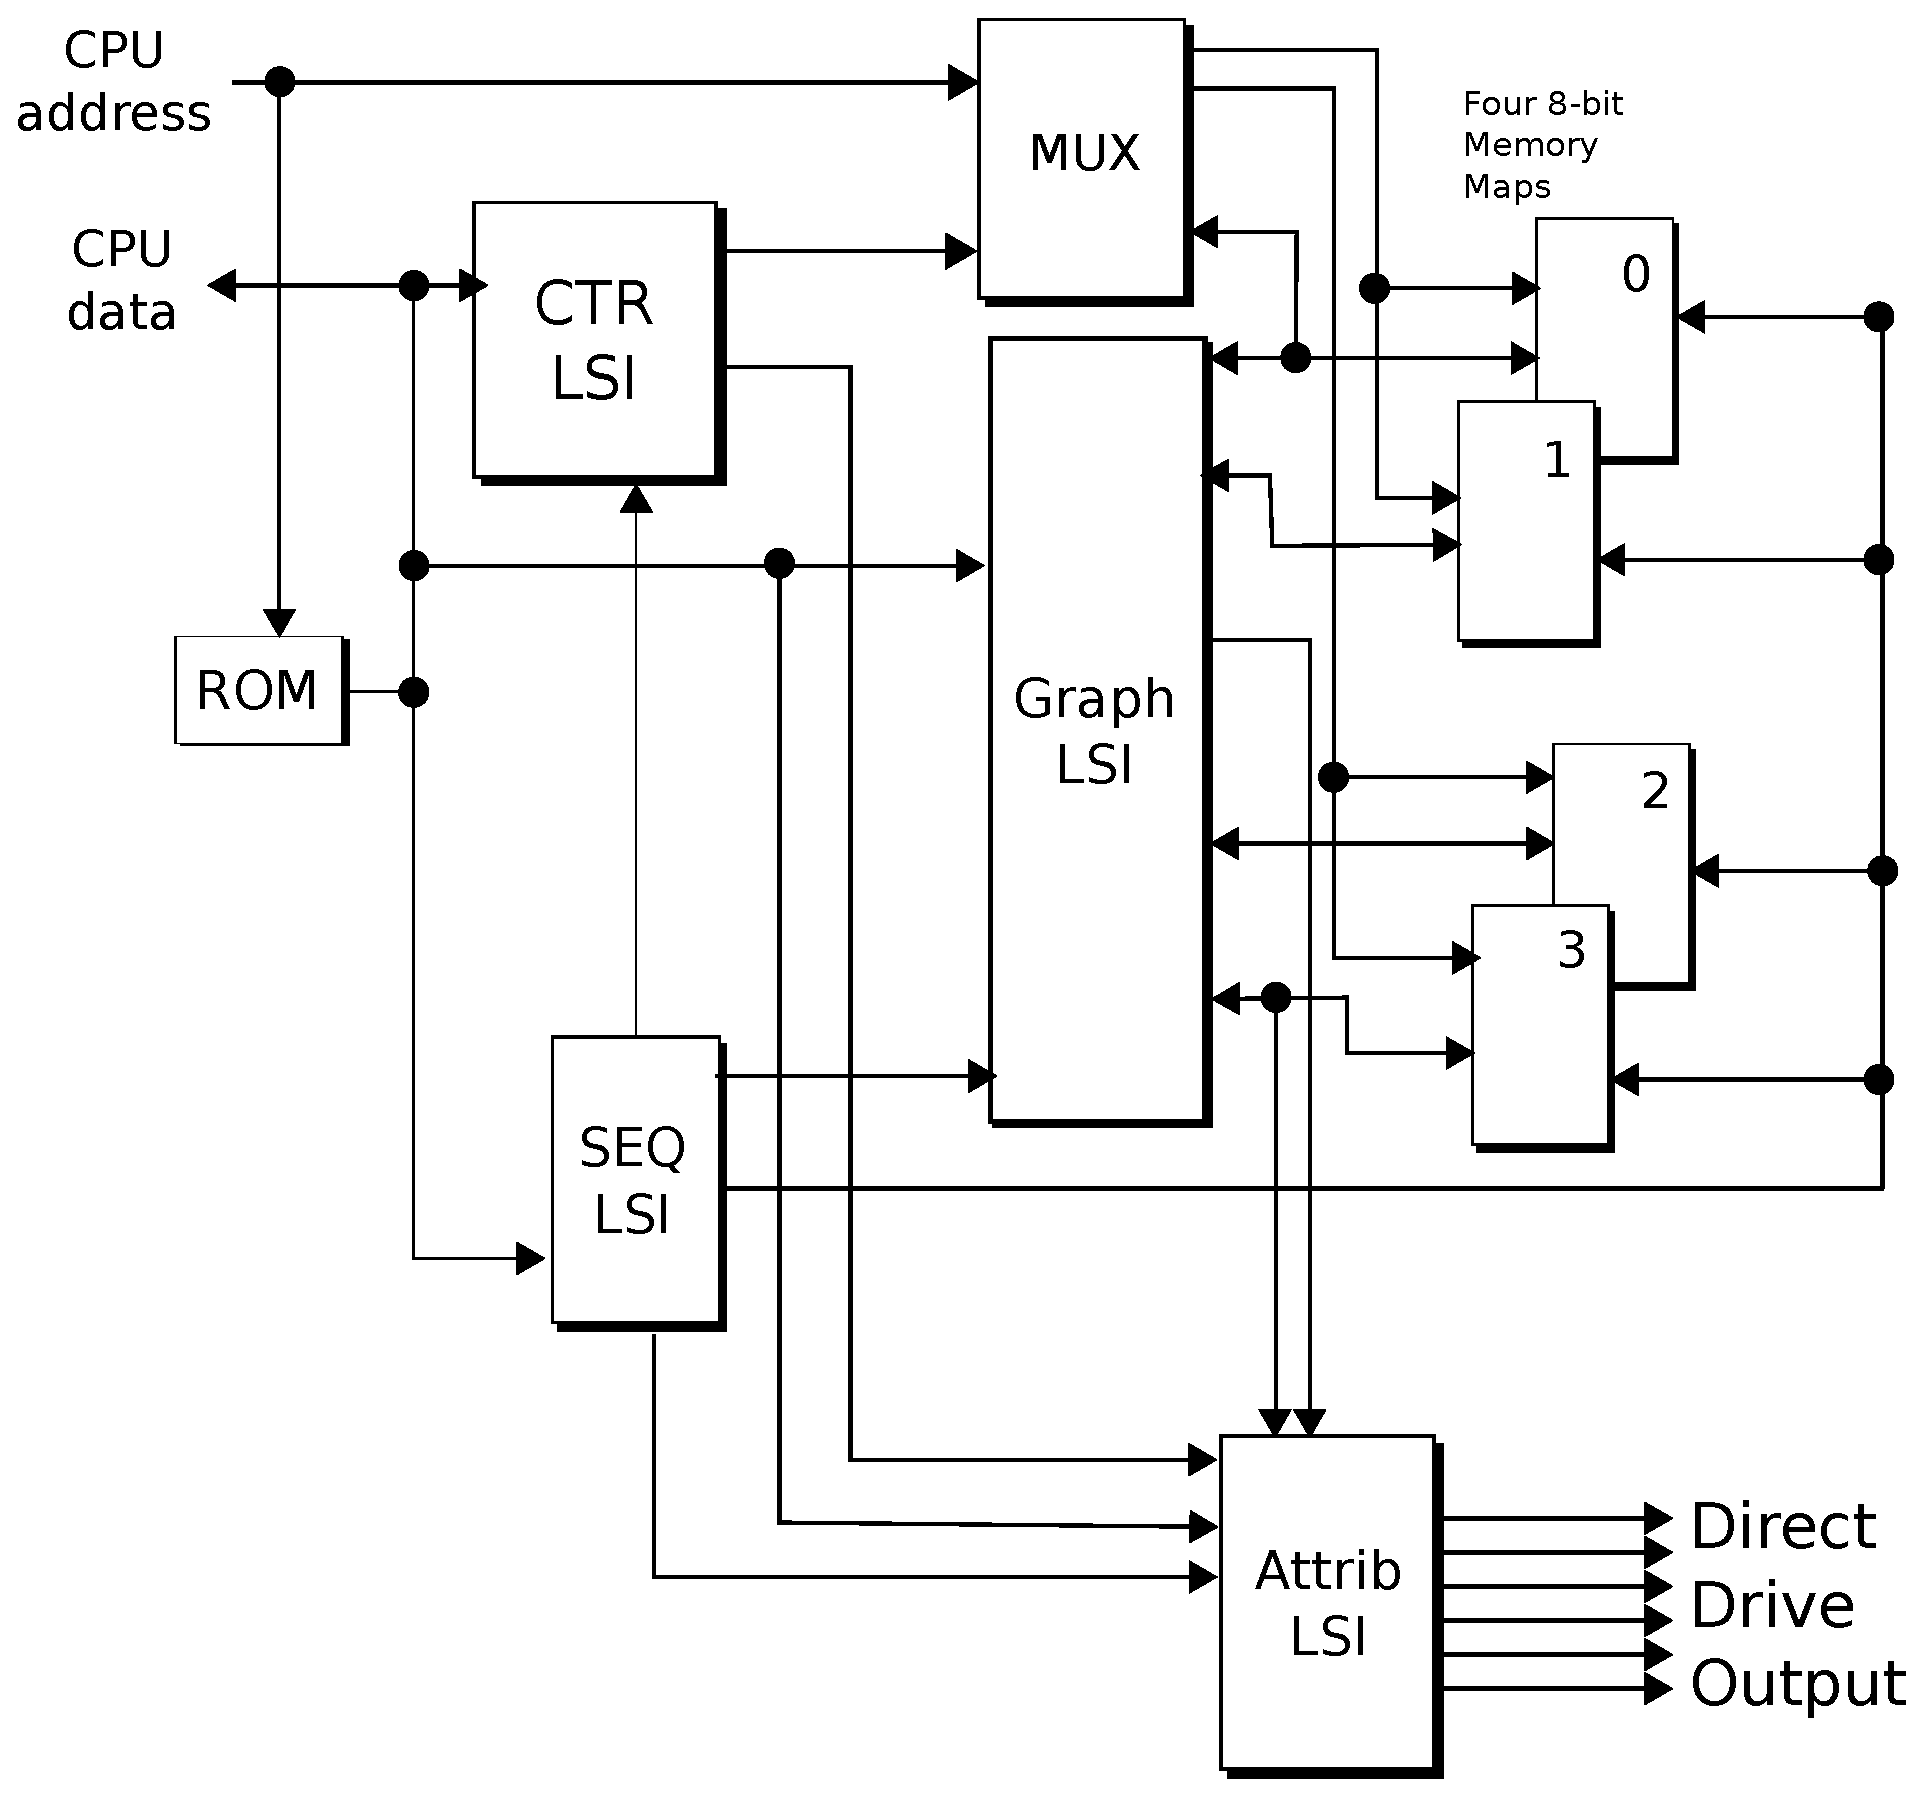
\includegraphics[width=\textwidth]{imgs/drawings/ibm_ega.eps}
\caption{IBM's EGA Documentation.}
\label{fig:ibm_ega}
\end{figure}

\par
To compensate for the complexity, IBM provided a routine to initialize all the registers via one BIOS call. One mode can be selected out of 12 available with an associated resolution, number of colors, and memory layout. The BIOS can be called to configure the EGA as follows:
\vspace{-10pt}
\begin{figure}[H]
\centering
\begin{table}[H]
\begin{tabularx}{\textwidth}[c]{llllcr}
\hline
\textbf{Mode} & \textbf{Type} & \textbf{Format} & \textbf{Colors} & \hspace{10pt}\textbf{RAM Mapping}\hspace{10pt} & \textbf{Hz}        \\ \hline
00h             & text          & 40x25           & 16 (monochrome) & B8000h     & 60                           \\ \hline
01h             & text          & 40x25           & 16              & B8000h    & 60                            \\ \hline
02h             & text          & 80x25           & 16 (monochrome) & B8000h    & 60                            \\ \hline
03h             & text          & 80x25           & 16              & B8000h    & 60                            \\ \hline
04h             & CGA Graphics  & 320x200         & 4               & B8000h    & 60                            \\ \hline
05h             & CGA Graphics  & 320x200         & 4 (monochrome)  & B8000h    & 60                            \\ \hline
06h             & CGA Graphics  & 640x200         & 2               & B8000h    & 60                            \\ \hline
07h             & MDA text      & 9x14            & 3 (monochrome)  & B0000h    & 60                            \\ \hline
0Dh           & EGA graphic   & 320x200         & 16              & A0000h    & 60                            \\ \hline
0Eh           & EGA graphic   & 640x200         & 16              & A0000h    & 60                            \\ \hline
0Fh           & EGA graphic   & 640x350         & 3               & A0000h    & 60                            \\ \hline
10h           & EGA graphic   & 640x350         & 16              & A0000h    & 60                            \\ \hline
\end{tabularx}
\end{table}
\caption{EGA Modes available.}
\label{ega-modes-available}
 \end{figure}
 
\trivia{The Modes \cw{08h-0Ah}  are reserved for PCjr (or Tandy Graphics Adapter) graphics modes, which offered 160x200 with 16 colors, 320x200 with 16 colors and 640x200 with 4 colors. Modes \cw{0Bh} and \cw{0Ch} are reserved for internal EGA BIOS.}\\

\par
To setup the EGA in Mode \cw{0Dh} using the BIOS is incredibly easy. It can be done with only two instructions:\\
  \par
  \lstinputlisting[ language={[x86masm]Assembler}]{code/ega_mode0d.c}
  
  \par
  The \codeword{geninterrupt (0x10)} instruction is a software interrupt caught by the BIOS routine in charge of graphic setup. It looks up the \codeword{ax} register, which can be set in the Borland Compiler by \codeword{\_AX}, to setup all EGA registers with the corresponding mode.\\
  
  \subsection{EGA Programming: Memory Mapping}
 \label{section:ega_memmap}
To write to the VRAM, the RAM's 1MiB address space maps 64KiB starting as indicated in figure \ref{ega-modes-available}. In mode \cw{0Dh} for example, the VRAM is mapped from 0xA0000 to 0xAFFFF. One of the first questions to come to mind is "How can I access 256KiB of RAM with only 64KiB of address space?" The answer is "bank switching" as summarized in figure \ref{ram_to_ega_mapping_label}. Write and Read operations are routed based on a mask register indicating which bank should be read or written to. \\



\begin{figure}[H]
  \centering
  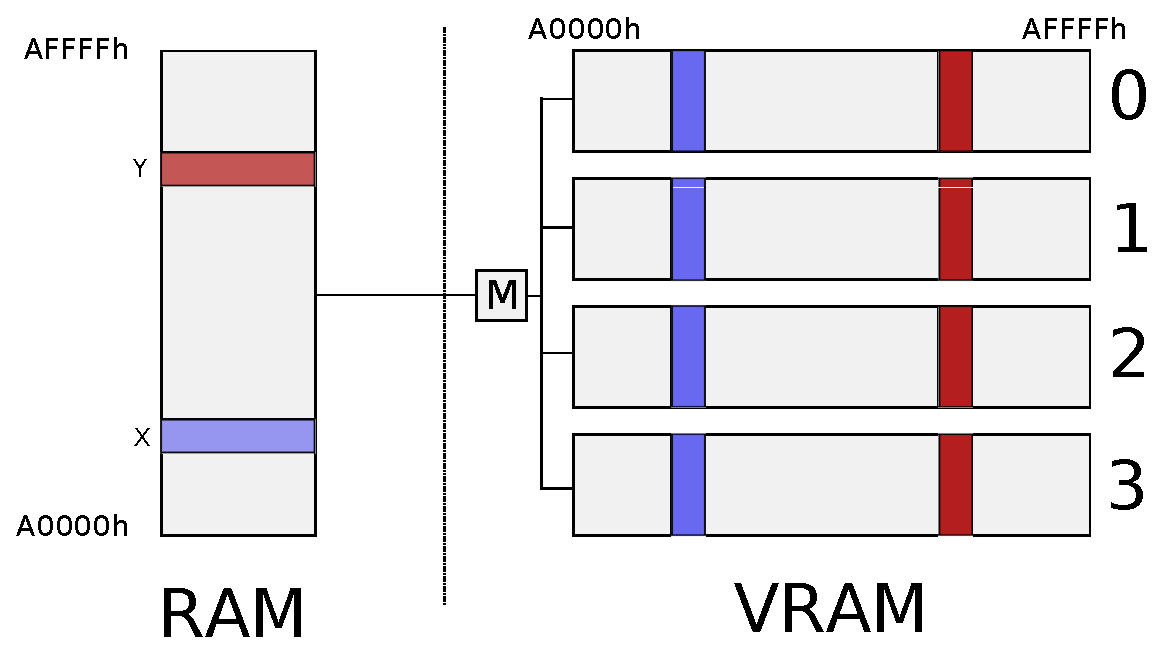
\includegraphics[width=.8\textwidth]{imgs/drawings/ram_to_ega_mapping.eps}
  \caption{Mapping PC RAM to EGA VRAM banks.}
  \label{ram_to_ega_mapping_label}
\end{figure}
\par
 
  
\subsection{EGA Color Palette}
\label{sec:ega_color_palette}
The EGA CRTC does not expect RGB values to generate pixels. Instead it is based on an index-based color palette system. Each pixel is a 4-bit index number, assigned to a color from the Attribute Controller. The default color palette are all 16 CGA colors, but it allows substitution of each of these colors with any one from a total of 64 colors.\\

When calculating the intended value in the 64-color EGA palette, the 6-bit number of the intended entry is of the form "rgbRGB" where a lowercase letter is the least significant bit of the channel intensity (\(\frac{1}{3}\) color intensity) and an uppercase letter is the most significant bit of intensity (\(\frac{2}{3}\) color intensity). The more intensity, the brighter the color is. For example, \cw{02h} will produce green, \cw{10h} will produce dim green and \cw{12h} will produce bright green. The color magenta is created by setting both "R" and "B", which is color code \cw{05h}. Each of the 16 color indexes could be reassigned to one color from the "rgbRGB" palette.\\


\begin{figure}[H]
\centering
\setlength{\tabcolsep}{2.8pt} % set border margin to 0
\begin{tabular}{|c|c|c|c|c|c|c|c|c|c|c|c|c|c|c|c|c|}
\hline 
 & 00h & 01h & 02h & 03h & 04h & 05h & 06h & 07h & 08h & 09h & 0Ah & 0Bh & 0Ch & 0Dh & 0Eh & 0Fh \\ \hline
 00h & \cellcolor{CGA_Black} & \cellcolor{CGA_Blue} & \cellcolor{CGA_Green} & \cellcolor{CGA_Cyan} & \cellcolor{CGA_Red} & \cellcolor{CGA_Magenta} & \cellcolor{EGA_06} & \cellcolor{CGA_Light_Grey} & \cellcolor{EGA_08} & \cellcolor{EGA_09} & \cellcolor{EGA_0A} & \cellcolor{EGA_0B} & \cellcolor{EGA_0C} & \cellcolor{EGA_0D} & \cellcolor{EGA_0E} & \cellcolor{EGA_0F} \\ \hline

10h & \cellcolor{EGA_10} & \cellcolor{EGA_11} & \cellcolor{EGA_12} & \cellcolor{EGA_13} & \cellcolor{CGA_Brown} & \cellcolor{EGA_15} & \cellcolor{EGA_16} & \cellcolor{EGA_17} & \cellcolor{EGA_18} & \cellcolor{EGA_19} & \cellcolor{EGA_1A} & \cellcolor{EGA_1B} & \cellcolor{EGA_1C} & \cellcolor{EGA_1D} & \cellcolor{EGA_1E} & \cellcolor{EGA_1F} \\ \hline

20h & \cellcolor{EGA_20} & \cellcolor{EGA_21} & \cellcolor{EGA_22} & \cellcolor{EGA_23} & \cellcolor{EGA_24} & \cellcolor{EGA_25} & \cellcolor{EGA_26} & \cellcolor{EGA_27} & \cellcolor{EGA_28} & \cellcolor{EGA_29} & \cellcolor{EGA_2A} & \cellcolor{EGA_2B} & \cellcolor{EGA_2C} & \cellcolor{EGA_2D} & \cellcolor{EGA_2E} & \cellcolor{EGA_2F} \\ \hline

30h & \cellcolor{EGA_30} & \cellcolor{EGA_31} & \cellcolor{EGA_32} & \cellcolor{EGA_33} & \cellcolor{EGA_34} & \cellcolor{EGA_35} & \cellcolor{EGA_36} & \cellcolor{EGA_37} & \cellcolor{CGA_Dark_Grey} & \cellcolor{CGA_Bright_Blue} & \cellcolor{CGA_Bright_Green} & \cellcolor{CGA_Bright_Cyan} & \cellcolor{CGA_Bright_Red} & \cellcolor{CGA_Bright_Magenta} & \cellcolor{CGA_Bright_Brown} & \cellcolor{CGA_White} \\ \hline


\end{tabular}\\
\setlength{\tabcolsep}{6pt} % reset border margin
\caption{EGA "rgbRGB" color palette (64 values from 00h to 3Fh)}
\end{figure}

\medskip
\par
However, standard EGA monitors did not support use of the extended color palette in 200-line modes. Both CGA and EGA cards use a female nine-pin D-subminiature (DE-9) connector for output. 
The EGA monitor could only distinct EGA and CGA cards based on the Vertical Sync signal, which is either 200- or 350-line mode. If the Vertical Sync is 350-line mode, the monitor switched to Mode 2 operations which supported the extended rgbRGB-color information\footnote{IBM Enhanced Color Display documentation.}. But in the 200-line mode, the monitor cannot distinguish between being connected to a CGA or an EGA card. \\




\par
The CGA color output is based on the form "RGBI", where the 'I' stands for Intensity and adds brightness to the RGB color. Compared to CGA, EGA redefines some pins of the DE-9 connector to carry the extended rgbRGB-color information. If the monitor were connected to a CGA card, these pins would not carry valid color information, and the screen might be garbled if the monitor were to interpret them as such. \\



\begin{figure}[H]
\renewcommand{\arraystretch}{0.7}
\centering
\begin{table}[H]
\begin{tabularx}{\textwidth}[c]{|>{\hsize=.16\hsize}X |>{\hsize=.42\hsize}X |>{\hsize=.42\hsize}X |}
\hline
\color{black} \textbf{Pin} & \color{black} \textbf{Mode 2: EGA mode (rgbRGB)} & \color{black} \textbf{Mode 1: CGA mode (RGBI)} \\
\hline
\color{black} 1 & \color{black} Ground &\color{black} Shield Ground \\
\hline
\color{black} 2 & \color{white}\cellcolor{EGA_I_Red} Secondary Red (Intensity) &\color{black}Signal Ground \\
\hline
\color{black} 3 & \color{white}\cellcolor{CGA_Red} Primary Red &\color{white}\cellcolor{CGA_Red} Red \\
\hline
\color{black} 4 & \color{black}\cellcolor{CGA_Green} Primary Green &\color{black}\cellcolor{CGA_Green} Green \\
\hline
\color{black} 5 & \color{white}\cellcolor{CGA_Blue} Primary Blue &\color{white}\cellcolor{CGA_Blue} Blue \\
\hline
\color{black} 6 & \color{black}\cellcolor{EGA_I_Green} Secondary Green (Intensity) &\color{white}\cellcolor{CGA_Dark_Grey}Intensity \\
\hline
\color{black} 7 & \color{white}\cellcolor{EGA_I_Blue} Secondary Blue (Intensity) &\color{black}Reserved \\
\hline
\color{black} 8 & \color{black} Horizontal Sync &\color{black}Horizontal Sync \\
\hline
\color{black} 9 & \color{black} Vertical Sync &\color{black}Vertical Sync \\

\hline

\end{tabularx}
\end{table}
\caption{EGA and CGA DE-9 connector pin signals.}
\label{pin_signals}
 \end{figure}
 

\par
Suppose one assigns the color brown (rgbRGB is \cw{010100b}) to one of the color indexes, the resulting color on the CGA pin assignment is light red; The secondary green pin ("r" in rgbRGB) is mapped to the Intensity pin in CGA mode, which results to the color red with intensity and not the expected brown color. \\

\par
For this reason, EGA monitors will use the CGA pin assignment (mode 1) in 200-line modes so the monitor can also be used with a CGA card and vice versa. Therefore, the EGA card is fully backwards compatible with a standard CGA monitor. Thereby it is able to show all 16 CGA (RGBI-)colors simultaneously, instead of only 4 colors when using a CGA card.  \\




\begin{figure}[H]
\renewcommand{\arraystretch}{0.7}
\centering
\begin{table}[H]
\begin{tabularx}{\textwidth}[c]{+X +X +X +X }
\hline
\textbf{\color{black}Index Number} & \textbf{\color{black}Color} & \textbf{\color{black}rgbRGB} & \textbf{\color{black}RGBI} 	\\ \hline
\rowcolor{CGA_Black}\rowstyle{\color{white}} 00h & Black          & 000000b           & 0000b 	\\ \hline
\rowcolor{CGA_Blue} 01h & Blue          & 000001b           &  0010b  			\\ \hline
\rowcolor{CGA_Green} 02h & Green          & 000010b           & 0100b   			\\ \hline
\rowcolor{CGA_Cyan} 03h & Cyan          & 000011b           & 0110b   			\\ \hline
\rowcolor{CGA_Red} 04h & Red          & 000100b           & 1000b   				\\  \hline
\rowcolor{CGA_Magenta} 05h & Magenta          & 000101b           & 1010b   		\\ \hline
\rowcolor{CGA_Brown} 06h & Brown          & 010100b           & 1100b   		\\ \hline
\rowcolor{CGA_Light_Grey} 07h & Light grey          & 000111b           & 1110b	\\ \hline
\rowcolor{CGA_Dark_Grey} 08h & Dark grey          & 111000b           & 0001b   		\\ \hline
\rowcolor{CGA_Bright_Blue}\rowstyle{\color{black}} 09h & Bright blue          & 111001b           & 0011b   			\\ \hline
\rowcolor{CGA_Bright_Green} 0Ah & Bright green          & 111010b   & 0101b	\\ \hline
\rowcolor{CGA_Bright_Cyan} 0Bh & Bright cyan          & 111011b     & 0111b   			\\ \hline
\rowcolor{CGA_Bright_Red} 0Ch & Bright red          & 111100b           & 1001b			\\ \hline
\rowcolor{CGA_Bright_Magenta} 0Dh & Bright magenta          & 111101b           & 1011b   		\\ \hline
\rowcolor{CGA_Bright_Brown} 0Eh & Yellow          & 111110b           & 1101b	\\ \hline
\rowcolor{CGA_White} 0Fh & White          & 111111b           & 1111b   		\\ \hline
\end{tabularx}
\end{table}
\caption{Default EGA 16-color palette}
\label{default_ega_palette}
 \end{figure}




 

  



\subsection{The Importance of Double-Buffering}
Double buffering has been mentioned often while describing the hardware, but so far we have not reviewed why it is paramount to achieving smooth animation. With only one buffer the software has to work at exactly the frequency of the CRT (60Hz). Otherwise a phenomenon known as "tearing" appears. Let's take the example of an animation rendering a circle moving from the left to the right:
\par
\begin{figure}[H]
\centering
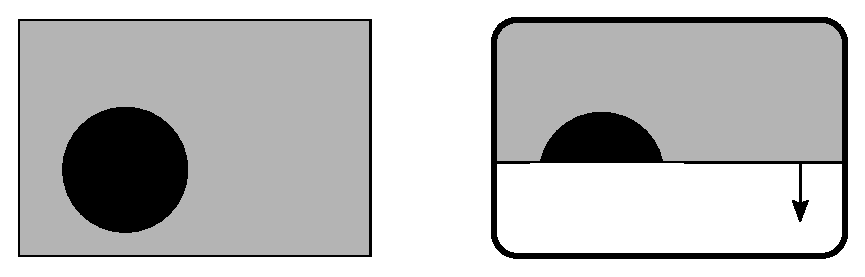
\includegraphics[width=\textwidth]{imgs/drawings/doublebuffer_before.eps}
\end{figure}
\par
In this example the CPU has finished writing the framebuffer (on the left) and the CRT's (on the right) electron beam has started to scan it onto the screen. At this point in time the electron beam has scanned half the framebuffer, so the circle has been partially drawn on the screen.
\par
\begin{figure}[H]
\centering
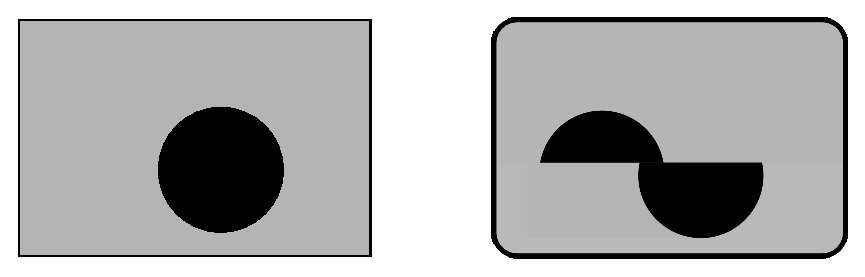
\includegraphics[width=\textwidth]{imgs/drawings/doublebuffer_after.eps}
\end{figure}
\par
If the CPU is faster than the frequency of the CRT (60Hz), it can write the framebuffer again, before the scan is completed. This is what happened here. The next frame was drawn with the circle moved to the right. The electron beam did not know that and kept on scanning the framebuffer. The result on screen is now a composite of two frames. It looks like two frames were torn and taped back together. Hence the name "tearing".\\

\par
With two buffers (a.k.a double buffering) the CPU can start writing in the second framebuffer without messing with the framebuffer being scanned to the screen\footnote{Now the CPU speed is capped by the CRT refresh rate. Triple buffering can solve this at the price of frame latency.}. No more tearing! A full screen of 320x200 pixels with 16 colors requires 320x200x 4-bits = 32KB of VRAM (spread over 4 planes, each 8KB), so there is plenty of video memory left to keep multiple screens in an EGA card with 256KiB memory.






\section{Audio}
\label{hardware-audio}
For the first 5-6 years of the IBM PC and its compatibles, their audio output came from nothing more than a simple loudspeaker with a tone generator. For business, this was acceptable - even preferable, since a PC in an office environment really shouldn't be a distraction to others! The loudspeaker, commonly known as a "PC Speaker", was capable of generating a square wave via 2 levels of output.\\
\begin{figure}[H]

\centering

\scaledimage{0.6}{pcspeaker.png}
\end{figure}


\subsection{History of Sound Cards}
The introduction of real game music and sounds on the PC started with Sierra back in 1988. They prepared to change all this by creating games that contained serious, high quality musical compositions drawing on add-on hardware. \textit{King's Quest IV} was the first commercially released game for IBM PC compatibles to support sound cards. In addition to the familiar PC speaker and Tandy 1000, it could utilize 
\begin{itemize}
    \item Roland MT-32
    \item IBM Music Feature Card
    \item AdLib
\end{itemize}
 
Sierra struck a deal with two companies, Roland and AdLib, where Sierra would also become a reseller for these soundcards. \\

\par
The Roland MT-32 was the higher end of these music devices. In today's terminology, it would be labeled a "Wavetable Synthesizer". A wavetable synthesizer usually implies that real instrument sounds are recorded into the hardware of the device. This device can then manipulate them to play them back at the various notes you need. The MT-32 had the ability to manipulate parts of its built in sounds using something called "Linear Arithmetic (LA)" synthesis. It was a very good device that can rival even today's sound cards. To connect the MT-32 to a PC required, what Roland called an MPU-401\footnote{Midi Processing Unit-401}, in one of the PC's expansion slots. Sierra sold The MT-32 with a necessary MPU-401 interface for \$550. The high price prevented it from dominating the end-user market of players.\\

\par
  \begin{figure}[H] 
    \centering 
    \scaledimage{.8}{hardware/MT_32.png} 
    \caption{Roland MT-32 synthesizer box.}
  \end{figure}


\par
The IBM Music Feature Card was launched in March 1987 as a collaboration between IBM and Yamaha. Essentially the Music Feature Card was a synthesizer installed on an 8-bit expansion card\footnote{Roland released the LAPC-I in 1989, which basically was similar to the Music Feature Card: a MT-32-compatible Roland sythesizer with a MPU-401 unit, integrated onto one single full-length 8-bit ISA card.}. The Music Feature Card had 8 FM voices, controllable via 4 frequency operators. It came with over 300 high-quality synthesized instruments on-board, and it was actually possible to have two Music Feature Cards in a single PC to get 16 voices! With a tag price of \$495 it was just like the Roland MT-32 an expensive card, and its audience was primarily business users.\\

\par
  \begin{figure}[H] 
    \centering 
    \scaledimage{1.0}{hardware/IBM_Music_Feature.png} 
    \caption{IBM Musice Feature Card.}
  \end{figure}

\par
  \bu{Trivia :} The IBM Music Feature Card was the very first general purpose "sound card" for the PC, beating AdLib by several months. \\


 \subsection{AdLib}
AdLib was the other company, beside Roland, that struck a deal with Sierra as a reseller. The company was founded in 1987 by Martin Prevel, a former professor of music from Quebec. The AdLib soundcard used a technology called FM synthesis. The technology is based on the idea of generating superimposing waveforms to create a sound. This technology was much less expensive than Roland's Wavetable technology.\\

\par
The AdLib card was built around the Yamaha YM3812, also known as the OPL2 chip, and could produce either 9 sound channels or 6 sound channels plus 5 hit instruments simultaneously using Frequency Modulation (FM). Ideally, if you have enough generators and can fine tune the waveforms well enough, you can create a realistic sound. However, to reach this ideal, you need lots of skilled people, lots of money for equipment, and lots of time to develop. The reality is, this is a cheap PC soundcard offering a better alternative than the PC Speaker. Thus, FM synthesis sounded very artificial. Still, this was a great improvement over the PC Speaker. With a price tag of \$219.99, it was much cheaper than the Roland MT-32 and IBM Music Feature Card, and soon ruled at the top of the early PC sound card market.\\

\par
  \begin{figure}[H] 
    \centering 
    \scaledimage{.8}{hardware/adlib.png} 
    \caption{An AdLib sound card. Notice the big YM3812 chip and the 8-bit ISA connector.}
  \end{figure}

\par
The AdLib card dominated the PC market for almost three years. In 1989, Creative Labs released the competing SoundBlaster, which quickly dominated over AdLib. To compete with SoundBlaster, AdLib planned a new 12-bit stereo sound card called AdLib Gold. Sadly, due to AdLib's dependence on Yamaha who suffered long delays introducing their latest multimedia chipset, their new product, AdLib Gold PC-1000, was never to see the light of day under AdLib's management. Unable to remain solvent, AdLib closed its doors on 1\textsuperscript{st} May 1992.\\




 
  


  \subsection{SoundBlaster}
  Creative Labs, the company behind the SoundBlaster, didn't enter the sound card industry until 1987 with the introduction of their Creative Music System (C/MS). From inception in 1981, they were a computer repair shop in Singapore. Creative Music System, or "Game Blaster" as it was renamed a year later, was an FM synthesizer card similar to AdLib. Based on the Philips SAA1099 chip which was essentially a square-wave generator, it sounded much like twelve simultaneous PC speakers would have, except for each channel having amplitude control. The card did not sell well.\\
  
  \par
The original Sound Blaster v1.0 and v1.5 were released in 1989 as the successor to their Game Blaster. Not only was it equipped with the OPL2 chip, providing 100\% compatibility with AdLib music playback, but it was also technologically superior with a DSP\footnote{An Intel MCS-51 "Digital Sound Processor", not "Digital Signal Processor".} allowing PCM playback (digitized sounds) at 8 bits per sample and up to 22.05kHz sampling rate. The card also came with a DA-15 port allowing joystick connection. Most importantly, the SoundBlaster was \$90 cheaper than the AdLib.\\


\par
\bu{Trivia:}
Creative Labs boasts in their own advert AdLib compatibility and even uses an image of AdLib Inc's product\footnote{Advert p20 in Compute!, April 1990.}! On the other hand they sued every company that tried to market a 'Sound Blaster compatible' product for using the name of their product.\\


\begin{figure}[H] 
  \centering 
  \fullimage{hardware/Soundblaster-ct1320.png} 
  \caption{A SoundBlaster 1.5, model CT1320B }
  \label{asb15}
\end{figure}

\par
Figure \ref{asb15} is the SoundBlaster model CT1320B. Notice the OPL2 chip (labeled FM1312) and the CT1321 DSP on the middle top. In the middle of the card are the two CMS-301 chips, to ensure backwards compatbility with the Creative Music System.\\

\par
  \bu{Trivia :} The CT1320B model (Sound Blaster 1.5) was a cost-cutting measure. Having recognised that C/MS was unpopular, they replaced the two C/MS chips with sockets. You could still purchase the C/MS chips for \$29.95 if you wished and install them into these sockets.\\


  \subsection{Disney Sound Source}
  The parallel port is nothing more than a way to pass out 8 bits simultaneously. Each PC had this port, and the conversion of this kind of data to an analogue signal is pretty simple and can either be achieved by using a DAC\footnote{Digital to Analogue Converter.} or simply a set of resistors. Hence the only thing missing was the interface, which a company named Covox delivered with their "Speech Thing" for only \$70.\\

\par  
   The difficulty about this sound device was to get exact timing. All bytes are converted the moment they reach the parallel port. In many ways it works pretty similar to the PC-speaker, only its connected to the parallel port. The CPU was in the center of all this, and it required lots of CPU resources to timely move information from RAM to the parallel port.  This left limited CPU time for the game or program, in a time period where the CPU already was the bottleneck.\\
   
  \par
  \begin{figure}[H] 
    \centering 
    \scaledimage{0.8}{hardware/ss.png} 
    \caption{The Disney Sound Source speaker box (DAC not shown).}
  \end{figure}
\par   
   
   \par
The Disney Sound Source came out around 1990 and fixed multiple issues: It contained a small buffer, so even an unsteady data stream resulted in a good audio signal. It also allowed to pass through the printer port, so there's no need to switch cables to print. And at \$14 it was dirt cheap! It came with its own amplifier, which ran with a 9 Volt battery. 


It would have made programmers and customers happy if not for one serious limitation: The buffer was fixed at a 7,000Hz, which is about the quality you get from an old fashioned phone. This was still enough to produce pleasant music, but fell short for sound effects when compared to AdLib and Sound Blaster.

\par
 \begin{figure}[H]
\centering
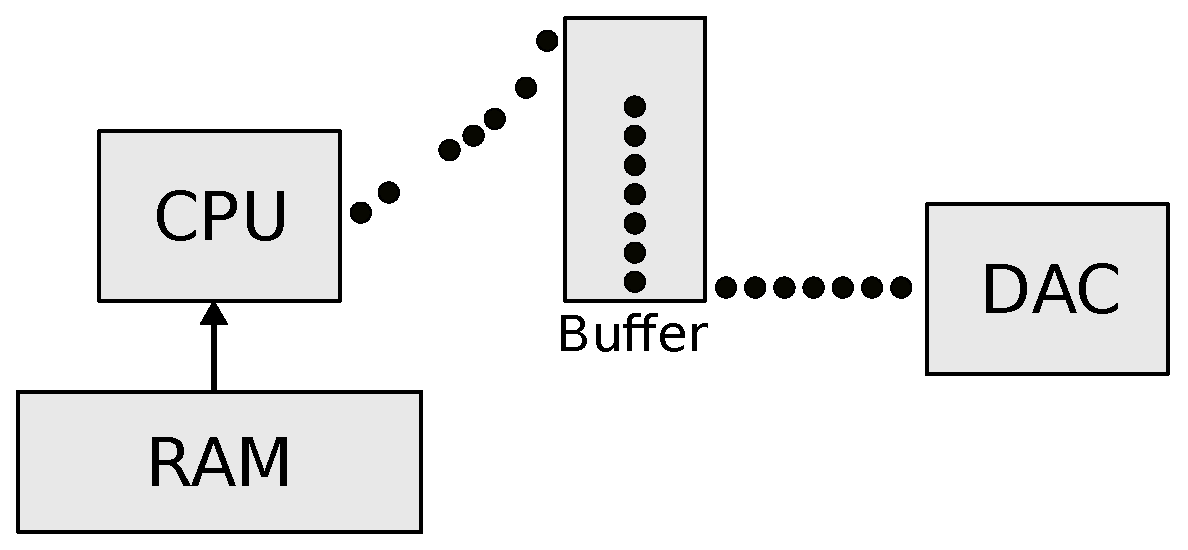
\includegraphics[width=0.7\textwidth]{imgs/drawings/DSS_buffer.eps}
\caption{Disney Sound Source with buffer, running at fixed 7,000Hz.}
\label{fig:DSS_buffer}
\end{figure}

  

\section{Floppy Disk Drive}
In the time before the internet, a floppy disk was the main medium to share and distribute software and data. The original XT systems were equipped with 5\nicefrac{1}{4}-inch floppy disk with a capacity of 360Kb. In 1984, IBM introduced with its PC AT the 1.2 MB dual-sided 5\nicefrac{1}{4}-inch floppy disk, but it never became very popular. IBM started using the 720 KB double density 3\nicefrac{1}{2}-inch floppy disk in 1986 and the 1.44 MB high-density version in 1987. The advantages of the 3\nicefrac{1}{2}-inch disk were its higher capacity, its smaller physical size, and its rigid case which provided better protection from dirt and other environmental risks. By the mid-1990s, 5\nicefrac{1}{4}-inch drives had virtually disappeared, as the 3\nicefrac{1}{2}-inch disk became the predominant floppy disk. \\

\vspace{10pt}
\bu{Trivia :} An USB stick of 128GB contains more than 91K high-density 3\nicefrac{1}{2}-inch (1.44MB) floppy disks.\\
\par

\begin{figure}[H]

  \begin{minipage}{0.48\textwidth}
  \centering
  \scaledrawimage{4cm}{hardware/floppy_3_1_2.png} 
  \end{minipage}
  \hfill
  \begin{minipage}{0.48\textwidth}
  \centering
  \scaledrawimage{6cm}{hardware/floppy_5_1_4.png}
  \end{minipage}
  \caption{3\nicefrac{1}{2}-inch and 5\nicefrac{1}{4}-inch floppy disk.}
  \end{figure}
\par


A floppy disk is essentially a very flexible piece (hence the term floppy disk) of plastic coated on both sides in a magnetic material. This 'disk' of plastic is contained within a protective envelope or hard plastic case, which is then inserted into the drive and automatically locked onto a spindle. It is then rotated at a constant speed, 360 rpm for standard PC floppy drives. A head assembly consisting of two magnetic read/write heads, one in contact with the upper surface and one in contact with the lower surface of the disk, may be moved in discrete steps across the disk and read the data from the disk.\\
\par
The floppy disk is controlled via the Floppy Disk Controller (FDC), a typical read operation from the floppy disk contains the following steps:
\begin{itemize}
  \item Turn the disk motor on. When you turn a floppy drive motor on, it takes quite a few milliseconds to "spin up", to reach the (stabilized) speed needed for data transfer.
  \item Perform seek operation, which moves the head to the correct location for reading the data.
  \item Read the data from the floppy disk and store the data via the FDC to RAM memory.
  \item Turn the disk motor off. 
\end{itemize}

The controller waited a few seconds before turning off the motor. The reason to leave the motor on for a few seconds is that the controller may not know if there is a queue of sector reads or writes that are going to be executed next. If there are going to be more drive accesses immediately, they won't need to wait for the motor to spin up again.\\




\section{Bus}
Although developers had no control over them, it is still worth mentioning how these components were connected to each other.\\ 
\par

The ISA\footnote{Industry Standard Architecture.} bus connects the CPU to all devices, including RAM. It was almost 10 years old in 1990 but still used universally in PCs. The data path to the RAM is 16 bits wide for 286 machines. It runs at the same frequency as the CPU.\\
\par

\begin{figure}[H]
\centering
      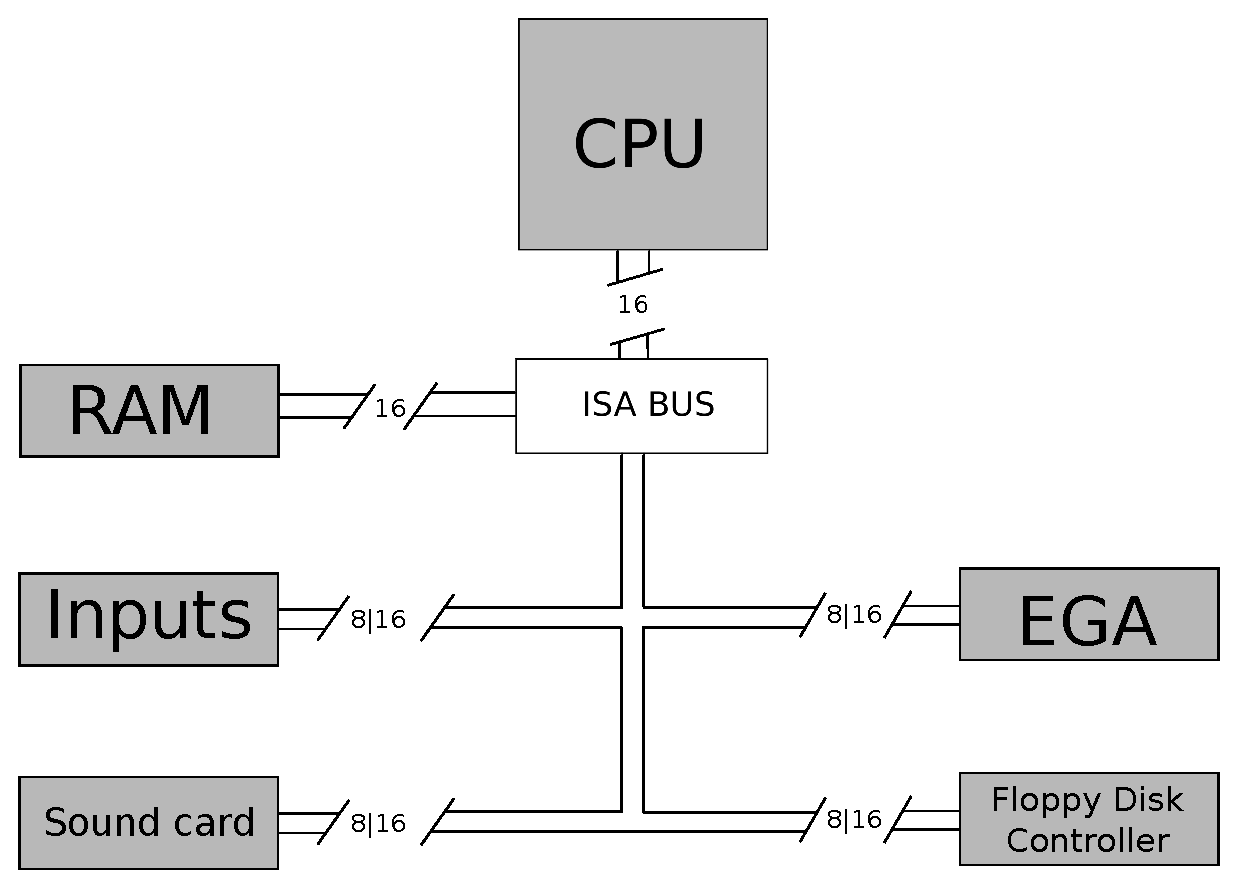
\includegraphics[width=0.9\textwidth]{imgs/drawings/bus.eps}
\end{figure}
\pagebreak
The rest of the bus connecting to everything that is not the RAM can be either:
\begin{itemize}
\item 8 bits wide at 4.77 MHz  for 19.1 Mbit/s
\item 16 bits wide at 8.33MHz for 66.7 Mbit/s\footnote{https://en.wikipedia.org/wiki/List\_of\_device\_bit\_rates .}.
\end{itemize}
It is also backward compatible and an 8-bit ISA card can be plugged into a 16-bit ISA bus.\\
\par
\vspace{10pt}
\bu{Trivia :} On ISA all devices are connected to the bus at all times and listen on the bus address lane. Each device features an "address decoder" to detect if it should reply to a bus request. This is how the EGA RAM is "mapped" in RAM. The EGA card "address decoder"  filters out everything that is not within \cw{A0000h} and \cw{AFFFFh}. Accordingly, the RAM disregards any request that is within the range [\cw{A0000h} - \cw{AFFFFh}].\\
\par
 \begin{figure}[H]
\centering
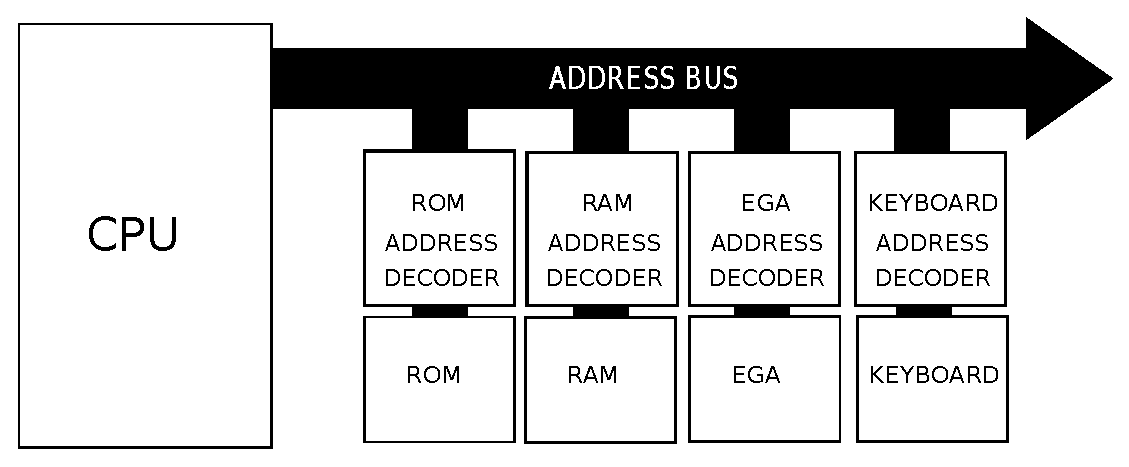
\includegraphics[width=\textwidth]{imgs/drawings/isa.eps}
\end{figure}







\section{Inputs}
At a time before the ubiquitous USB, inputs were a mess with no less than four ports, all programmed differently.\\

The parallel port (DB-25) was on every computer and usually used to connect dot-matrix printers (loud things that printed with needles). The parallel port was multi-purpose and the Disney Sound Source could be plugged into it.\\
\par
 \begin{figure}[H]
\centering
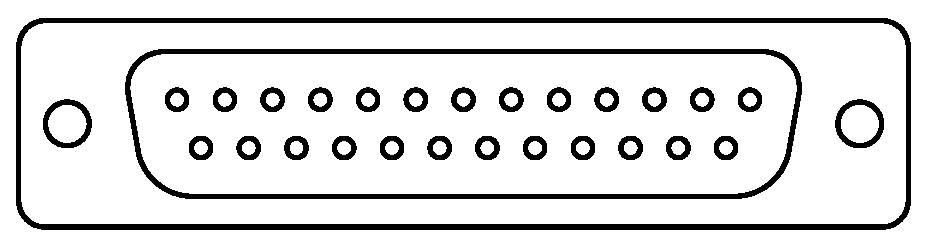
\includegraphics[width=0.3\textwidth]{imgs/drawings/ports/DB-25_parallel_port.eps}
\caption{Parallel Port}
\label{fig:parallelPort}
\end{figure}


The serial port (DE-9) was used to connect the mouse. The EGA monitor is also using a DE-9 connector, so it happened that people tried to plugin a mouse into the EGA card.
 \begin{figure}[H]
\centering
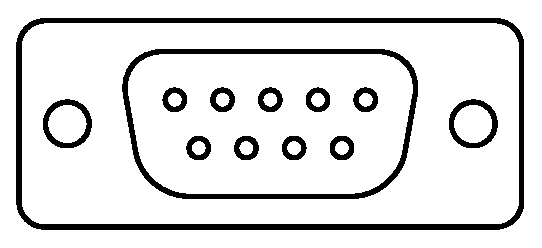
\includegraphics[width=0.15\textwidth]{imgs/drawings/ports/DE9_serial_port.eps}
\caption{Serial Port and EGA Port}
\label{fig:serialPort}
\end{figure}


The PS/2 port was used to connect a keyboard.
 \begin{figure}[H]
\centering
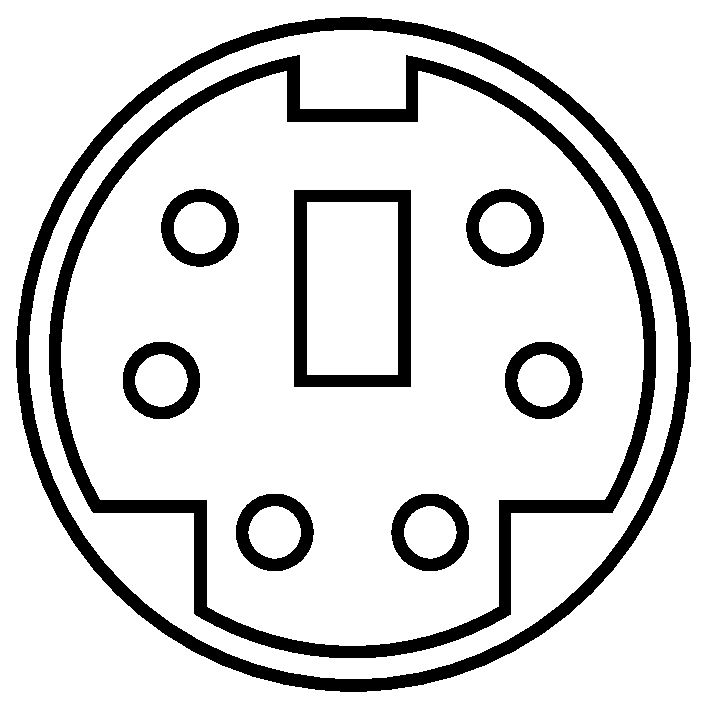
\includegraphics[width=0.07\textwidth]{imgs/drawings/ports/MiniDIN-6_PS2.eps}
\caption{PS/2 Port}
\label{fig:ps2Port}
\end{figure}


Finally, a SoundBlaster sound card connected via the ISA bus provided a Game Port (DA-15) allowing for connection to a joystick\footnote{In 1981, the very first IBM PC could be purchased with a DA-15 "Game Port" extension card at the cost of \$55 (\$159 in 2018).}.
 \begin{figure}[H]
\centering
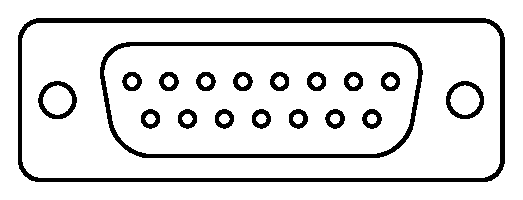
\includegraphics[width=0.19\textwidth]{imgs/drawings/ports/DA-15_GamePort.eps}
\caption{Game Port}
\label{fig:gamePort}
\end{figure}



\section{Summary}
To say a PC was difficult to program for games would be an understatement. It was a nightmare. The CPU was good at doing the wrong thing, the best graphic interface didn't allow double buffering, and the memory model only allowed 1 MiB with an address composed of two separate 16-bit registers. Last, but not least, the default sound system could only produce square waves.\\
\par
Yet despite all these unfavorable conditions, teams of developers gathered to tame the beast and unleash its power to gamers. One of these called themselves \textit{Ideas From the Deep}\footnote{They originally called themselves Ideas From the Deep but then decided to shorten it to simply id, which stands for "in demand", and is pronounced as in "did" or "kid." The name also refers to id, the part of the brain that behaves by the pleasure principle in Freudian psychology.}.
\end{document}




